\documentclass[a4paper]{article}

\usepackage[utf8]{inputenc}
% Citation
\usepackage[square,numbers]{natbib}

\usepackage{amsmath}
\usepackage{longtable}
\usepackage{graphicx}
\usepackage{fancyhdr}
\usepackage{tabularx}
\usepackage{listingsutf8}
\usepackage{lmodern}  % for bold teletype font
\usepackage{amsmath}  % for \hookrightarrow
\usepackage{xcolor}   % for \textcolor
\lstset{
  columns=fullflexible,
  frame=single,
  breaklines=true,
  postbreak=\mbox{$\hookrightarrow$\space},
}

\usepackage{amssymb}% http://ctan.org/pkg/amssymb
\usepackage{pifont}% http://ctan.org/pkg/pifont
\newcommand{\cmark}{\ding{51}}%
\newcommand{\xmark}{\ding{55}}%
\usepackage{hyperref}
\usepackage{etoolbox}% http://ctan.org/pkg/etoolbox
\usepackage{needspace}% http://ctan.org/pkg/needspace
\usepackage{amsthm}

% Code listings
\lstset{numbers=left, numberstyle=\tiny, basicstyle=\ttfamily, numbersep=5pt, breaklines=true}
\lstset{emph={square}, emphstyle=\color{red}, emph={[2]root,base}, emphstyle={[2]\color{blue}}}


\usepackage{array}
\newcolumntype{L}[1]{>{\raggedright\let\newline\\\arraybackslash\hspace{0pt}}m{#1}}
\newcolumntype{C}[1]{>{\centering\let\newline\\\arraybackslash\hspace{0pt}}m{#1}}
\newcolumntype{R}[1]{>{\raggedleft\let\newline\\\arraybackslash\hspace{0pt}}m{#1}}

\usepackage[colorinlistoftodos,prependcaption,textsize=tiny]{todonotes}

%\Bearbeitet Format, sodass statt der Einrückung bei Paragraphen durch Zeilenabstand ersetzt wird
\usepackage{parskip}
\setlength\parindent{0pt}

%\Setzt Dokumentinformationen
\title{\large Master-Thesis in Informationsmanagement und Informationstechnologie: \\ \Huge Incremental Analyses of Software Product Lines}
\author{Moritz Fl\"oter}
\date{June 2018}


\begin{document}
\pagenumbering{gobble}
\bibliographystyle{alpha}

\newtheoremstyle{mystyle}% name
  {3pt}%Space above
  {3pt}%Space below
  {\normalfont}%Body font
  {0pt}%Indent amount
  {\bfseries}% Theorem head font
  {}%Punctuation after theorem head
  {\newline}%Space after theorem head 2
  {}%Theorem head spec (can be left empty, meaning 'normal')

\theoremstyle{mystyle}


\newtheorem{req}{REQ}
\newtheorem{subreq}{REQ}[req]
\newtheorem{subsubreq}{REQ}[subreq]
\AtBeginEnvironment{req}{\Needspace{5\baselineskip}}
\setcounter{req}{0}

\newcommand*{\reqtable}[4]{
\begin{tabular}{ | p{0.15\textwidth} | p{0.79\textwidth} | }
	\hline
	\textit{Priority} & \begin{minipage}[l]{0.79\textwidth}
	\vspace{0.25em}
		#1
	\vspace{0.25em}
	\end{minipage} \\ \hline
	\textit{Source} & \begin{minipage}[l]{0.79\textwidth}
	\vspace{0.25em}
		#2
	\vspace{0.25em}
	\end{minipage}\\ \hline
	\textit{Description} & \begin{minipage}[l]{0.79\textwidth}
	\vspace{0.25em}
		#3
	\vspace{0.25em}
	\end{minipage} \\ \hline
	\textit{Explanation} & \begin{minipage}[l]{0.79\textwidth} 
	\vspace{0.25em}
		#4
	\vspace{0.25em}
	\end{minipage} \\
	\hline
\end{tabular}
}



%\Deckblatt
\maketitle
\newblock

\begin{center}
floeter@uni-hildesheim.de \par
Matrikel-Nr: 236278 \par
Supervisors: \par
Prof. Dr. Klaus Schmid \par
Christian Kr\"oher
\end{center}

\newpage
\lhead{{}}
\rhead{\leftmark}
\pagestyle{fancy}

\listoftodos[Notes]
\clearpage

\pagenumbering{roman}

\begin{verbatim}
\end{verbatim}
\Large \textbf{Eigenst\"andigkeitserkl\"arung} \normalsize


\textbf{Erkl\"arung \"uber das selbstst\"andige Verfassen von dieser Arbeit}

Ich versichere hiermit, dass ich die vorstehende Arbeit selbstständig verfasst und keine anderen als die angegebenen Hilfsmittel benutzt habe. Die Stellen der obigen Arbeit, die anderen Werken dem Wortlaut oder dem Sinn nach entnommen wurden, habe ich in jedem Fall durch die Angabe der Quelle bzw. der Herkunft, auch der benutzten Sekund\"arliteratur, als Entlehnung kenntlich gemacht. Dies gilt auch f\"ur Zeich\-nun\-gen, Skizzen, bildliche Dar\-stel\-lung\-en sowie f\"ur Quellen aus dem Internet und anderen elektronischen Text- und Datensammlungen und dergleichen. Die eingereichte Arbeit ist nicht anderweitig als Pr\"u\-fungs\-leis\-tung verwendet worden oder in deutscher oder einer anderen Spra\-che als Ver\-\"off\-ent\-lich\-ung erschienen. Mir ist bewusst, dass wahrheitswidrige Angaben als Täu\-schung behandelt werden.

Lehrte, den 29.06.2018


\unitlength 5mm
\begin{picture}(5,4) \put(0,0) {\line(1,0){22}} \end{picture}\\

 
\newpage

%\Inhaltsverzeichnis
\tableofcontents
\newpage
\bibliographystyle{unsrt}

%\Deckblatt
\maketitle
\newpage




% Continous counting of footnotes
\pagenumbering{arabic}
\setcounter{page}{1}
\lhead{{}}
\rhead{\leftmark}
\pagestyle{fancy}



\section{Introduction}

Software product lines offer a means to efficiently develop software by enabling the reuse of assets in different configurations. They reduce development and maintenance cost, enhance the quality and shorten development cycles \cite{Pohl:2005:SPL:1095605} \cite{Apel:2013:FSP:2541773} \cite{spl-in-action}. However they come with their own set of problems when it comes to testing, measuring or analyzing products as a product line can represent a staggering amount of configurable products. Assuming a product line with only ten independently selectable configuration options, we are already faced with 1024 configurable products. That means 1024 products that can potentially be analyzed. With 20 configuration options, this increases to over a million possible products. Even if not every single product is analyzed, the variety of possible configuration somehow has to be considered when perfoming analyses. Instead of focusing on the analysis of individually configured products, an analysis can also directly work with variability information which describes how different configurations are represented within the product line. Thereby the analysis can analyze the whole family of products described by a product line at once. Working with this information also allows analyses to analyze aspects specific to software product lines that do not occur within the development of single products outside of a product line.

While analyzing each individual product with an individual analysis is often not feasible, family based analyses that incorporate variability information allow similar analyses to be executed with significantly less computational effort. At the same time, family based analyses may allow similar conclusions as product based analyses for a given product configuration. Therefore family based analyses allow to make assumptions not only based on one product but on the entire product line. They do however still entail a considerable computational effort. As an example, the single threaded execution of the analysis that we use for evaluation purposes takes about eight hours per execution on current hardware. It would however be desirable to provide developers with timely feedback by performing analyses even faster.

The analyses performed by our IDEs or CI systems are examples of how analyses can support everyday implementation tasks. 
The continous syntax checking within IDEs is one example of an analysis that helps us to write correct code. And while parsing code usually does not entail any noteworthy performance drops during development, parsing code for product lines may be more difficult. This is because through conditional compilation, code fragments within sourcefiles of product lines can either included or removed. Therefore a source file can not be interpreted as one file delivering one outcome but must be processed considering multiple possible options. With SuperC, Gazzillo and Grimm \cite{gazzillo-grimm} developed a variability aware parser that allows to parse C-code including the compiler directives for the C-preprocessor that are used for conditional compilation. Thereby SuperC allows to perform syntactic analyses of C code while preserving variability. 

TypeChef implements type checking for product lines and helps to ensure that \emph{every} possible product is correctly typed. Type checking is usually performed by the compiler - for our relatively simple product line with 20 configuration options that would mean that more han one million products would need to be processed by the compiler. By using a variability aware type system, TypeChef is able to guarantee that the code is well typed for all variants \cite{Kenner:2010:TTT:1868688.1868693}.

The dead code analysis as implemented by Undertaker \cite{Tartler:2011:FCC:1966445.1966451} offers insight on the variability implementation itself. It is able to detect code segments that are never included in any configurable product due to constraints deduced from information about variability within the product line. This is relevant for developers as unused code segments result in additional maintenance effort and increase code complexity without contributing to configurable products.

As those examples for analyses show, analyses for software product lines may aid the development. While tools like SuperC or TypeChef already introduced performance benefits compared to the brute force analysis of every configurable product, they still entail a considerable computational effort. Research has shown that family-based strategies are still slower than the analysis of a single product \cite{Thum:2014:CSA:2620784.2580950}. However during development, timely feedback on currently modified artifacts is desirable. Therefore  improvements to the performance of software product line analyses are required.

This work aims to further reduce the required computational effort for performing analyses during development. It is meant to provide developers with timely feedback about their work and enable more frequent analyses. Our concept aims for a result covering every change introduced to the product line. When a developer commits changes into the repository of a software product line, he usually only changes a part of the existing files. We use the change information to provide analysis results on his modification instead of reanalyzing the entire product line for every commit. In some cases a developers changes might not even affect the results of the analysis. For example the addition of a comment has no effect on the configuration options of a product line and therefore does not require a new analysis if that is what the analysis is based on. We inspect the introduced change to determine whether or not it modifies information that affects the analysis result and then decide whether or not a new analysis needs to be performed. We refer to those analyses as incremental analyses.

Our concept for incremental analyses is based on the findings of an analysis of commits to the Linux Kernel. Kr\"oher and Schmid \cite{ComAn} created a technical report analyzing the nature of the changes introduced through commits to the Linux Kernel and Coreboot. They found that out of the 632.601 commits to the Linux Kernel that their analysis covered, only 66.635 commits introduced changes to variability. This means that if the result of an analyis for a software product line is entirely dependent on variability information, only about 9.49\% of commits would require an analysis to be performed. 

However, identifying variability changes introduces an additional step resulting in additional computational effort. Furthermore only considering files affected by variability changes for the analysis may produce deviations for the computed analysis result if does not purely depend on variability information. Therefore our implementation also includes an option to process all files affected by changes.  Kr\"oher and Schmid \cite{ComAn} showed that 78.29\% of commits to the Linux Kernel modified code files exclusively while files defining build and configuration remained untouched. Our tooling is able to perform partial analyses for such changes thereby only processing the newly introduced changes to codefiles.  Our implementation of an incremental dead code analysis uses change information to reduce the computational effort of the eanalysis. Therefore it represents the implementation of an evolutionary analysis as suggested by Kr\"oher et al. \cite{ComAn-splc}. 

Using the dead code analysis as an example for incremental analyses, we try to answer the following questions: Can we achieve similar results with our incremental approach compared to the non-incremental analysis approach? If the results differ - what is are the reasons?  Does the incremental approach provide performance benefits and how big are they?

This work is structured as follows: Chapter \ref{background} will introduce software product lines along with the Linux Kernel as an example. It will then cover software product line analyses and KernelHaven as an infrastructure for performing analyses on software product lines. Chapter \ref{requirements} lists the requrirements for our implementation. Chapter \ref{concept} will provide a brief introduction to the concept of incremental analyses that will then serve as foundation for the implmenentaion which is described in Chapter \ref{implementation}. Following this, Chapter \ref{evaluation} will cover the evaluation of the developed infrastructure for incremental analyses using the dead code analysis as an example. Finally Chapter \ref{threats-to-validity} will discuss threads to validity while Chapter \ref{conclusion} summarizes this works and provides perspectives for future research.


\section{Background} \label{background}

This section will introduce software product lines and the Linux Kernel  specifically. This builds the foundation for understanding analyses on software product lines that are introduced subsequently. Before diving into the concepts of incremental analyses in the following chapters, the software project KernelHaven is introduced as an infrastructure for performing analyses on software product lines. KernelHaven itself will be used as the foundation for the practical implementation of our approach.

\subsection{Software Product Lines}\label{spl}

When starting a new software project from scratch, one approach is to write code specifically for that project. The codebase and the documentation are tailored to the needs and requirements currently at hand. And when another project is to be implemented, you do the same thing there. However it might turn out that those two projects technically share common functionality eventhough each product has features that the other does not.

For related projects, instead of writing code for one project specifically it might have made sense to create something that is configurable to cover multiple use-cases across different projects. Then for the next project it would be possible to combine and configure existing developed artifacts. And after some more projects it is perhaps even possible to realize a new product just by configuring and combining the assets that have already been created. This is where software product lines come in. In contrast to traditional software development, softwae product lines aim to reuse existing assets instead of writing software from scratch.

Software product lines use engineering techniques for creating a portfolio of similar systems from a shared set of software assets \cite{intro-spl}. This differenciates software product lines from software systems with \emph{opportunistic} reuse. \emph{Oppurtunistic} reuse of single components occurs in many software projects where parts of an developed system are reused by other components or included as library within other projects. However software product lines are actively built for reuse, thereby employing a \emph{predictive} reuse system, that directly aims for future products to be able to reuse created assets.

While considering configurability and reusability of assets when developing a single product results in a higher initial effort, the break even point is usually reached after about three products. Therefore incorporating the principles of software product lines is advantageous when multiple system are able to share the same assets. Through the reuse of existing assets across multiple products, the development, maintainance and documentation effort is drastically reduced. Furthermore a new product is most likely more reliable and secure as it can be built directly on top of mature components  \cite[p.4f]{spl-in-action}. Within a software product line, a \emph{configuration} is a selection of options that define how a product behaves. A configuration can be used to create a product that is the result of selected configuration options.

Because products in product lines can be configured to match specific requirements, each product posesses a distinct set of characteristics. The characteristics implemented within of a product line can be differenciated into three types called variability types \cite[p.8]{spl-in-action}:
\begin{description}
\item[Commonality]  A characteristic that is shared across all members of the product line.
\item[Variability]  A characteristic that is included in some, but not all members of the product line.
\item[Product-specific]  A characteristic that is only included within one product. 
\end{description}

Kang et al. \cite{KangFeatureOrientedDomain1990} define a \emph{feature} as an end-user visible characteristic of a system. Features define both common aspects as well as differences between related systems. Therefore features describe certain aspects of variability within a software product line. Features within a software product line can be visualized using a feature model diagram as shown in \autoref{featuremodel}. 

\begin{figure}[h] 
  \centering
  \begin{minipage}[b]{1\textwidth} 
    \caption[Feature Model]{Feature Model for an Operating System}\label{featuremodel}
    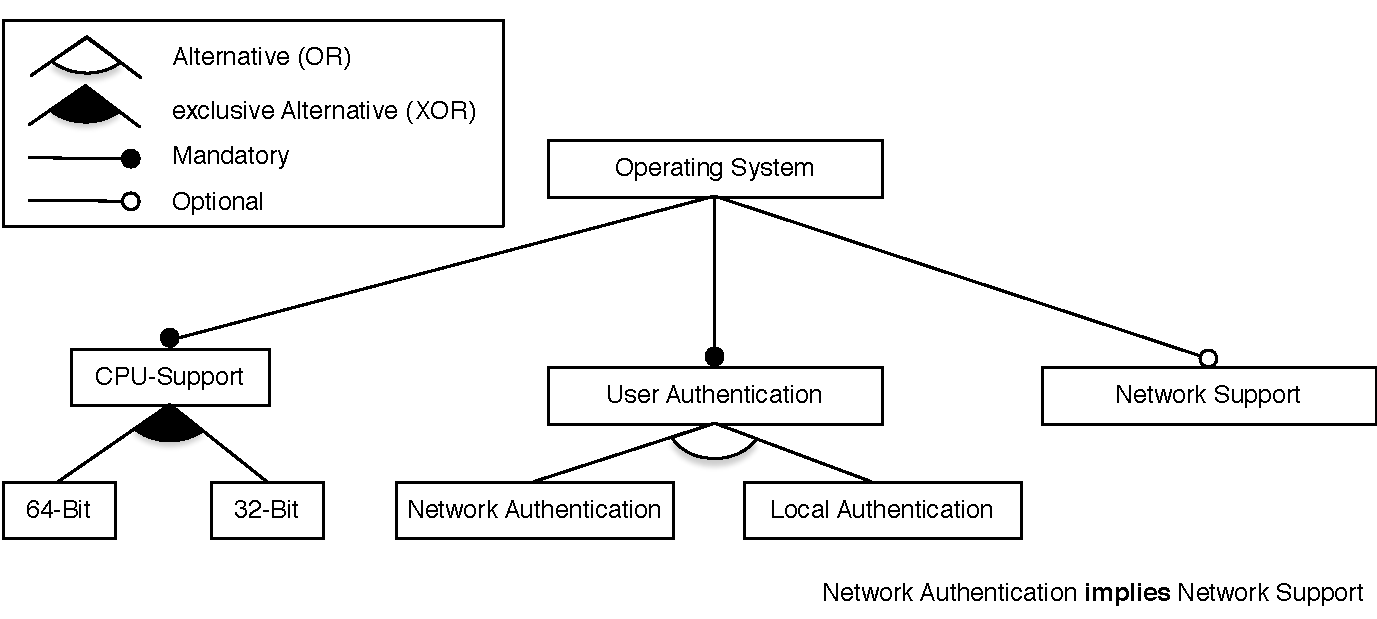
\includegraphics[width=1\textwidth]{img/featuremodel.pdf}
  \end{minipage}
\end{figure}

In the example, the operating system has to include support for a CPU through either a 32-Bit or 64-Bit option. While CPU-Support itself is a mandatory feature, the choice between the 32-Bit and 64-Bit option is an exclusive one. When choosing one option, the other option can not be included. The selection of both Network Authentication and Local Authentication is however possible for the User Authentication feature as the choice between them is not exclusive. However Network Authentication requires the selection of Network Support (indicated at the bottom right corner of \autoref{featuremodel}) which would otherwise be an optional feature. The feature model is only one example of how variability within a software product line can be represented. Another textual representation of variability will be introduced in Section \ref{linux-kernel} in the context of the Linux Kernel. It is worth noting that the Linux Kernel uses a decision model instead of a feature model to model variability.

\emph{Variability models} represent configuration options and their dependencies as variables and constraints between them. A variability model thereby defines possible combinations of configuration options. However the variability model does not represent how configured options are translated into the final product. In order to cover this process as well, we use two other models, the build and the code model. The \emph{build model} describes the build process and thereby maps a concrete configuration to code files. The code model on the other hand represents variability on the level of source code. The consideration of three components related to handling variability within a product line can also be found in previous work covering the Linux Kernel  \cite{nadi-linux-kernel} \cite{mining-kbuild} and C-Preprocessor based product lines in general \cite{KroeherEl-SharkawySchmid18}.

The \emph{build model} represents how a concrete configuration is realized when building a product. A build system automates the process of program compilation. Its primary task is to create executables. For the build system of software product line this means that it can carry the responsibility for selecting or even modifying compilation targets according to a concrete configuration. Following our example, the source-files related to the Network Support feature only need to be included into the build when the feature has been selected. The generic elements for the CPU-Support Feature on the other hand must be included at all times as they are a commonality for the product line. 

As the selective compilation of source code is a mechanic that works before or at compilation time, it represents the implementation of \emph{compile-time variability}. This is however not the the only option for achieving variability within a product. Another option is to modify the product is started (\emph{load-time variability}) or executed (\emph{run-time variability}) \cite[p.49]{Apel:2013:FSP:2541773}. It is for example possible to include more than one user interface for the same product and allow the user to select his preference even after the product has been compiled. While all three approaches allow the configuration of features within a within a software project, they differ in the binding-time of the feature. 

Finally different behaviours depending on the configured options for a product may also be defined through the source code. This can be achieved by using conditional compilation. In conditional compilation, compiler directives are used to include or exclude code sections from compilation. 

Before diving into technical details, the terminology used for the remainder of this work needs some clarification. The set of all files  that represent a software system and are used as input for an analysis will be referred to as the codebase. The codebase therefore includes files containing source code as well as files defining the build process or configuration-options. The terms source file or code file on the other hand will be used in their usual interpretation and refer to a file that contains source-code. Finally variability model files and build model files are files within the codebase that relate to the respective models. 

\subsection{The Linux Kernel}\label{linux-kernel}

In this section, we will take a closer look at how variability is incorporated in the Linux Kernel project. The Linux Kernel is a prominent example of a software product line in the operating system domain. The Linux Kernel handles variability utilizing the conditional compilation of the C-Preprocessor as a core component.  Eventhough other C-Preprocessor based software product lines exist, many of them stem from a commercial context and are closed-source while the Linux Kernel is an open-source project. In order to enable the reproduction of our results as well as accessibility to the components used for this work, the Linux Kernel was chosen as target for evaluating the developed incremental analysis. The Linux Kernel itself comes with more than 10.000 configurable features \cite{Tartler:2011:FCC:1966445.1966451}. 

\begin{figure}[h] 
  \centering
  \begin{minipage}[b]{1\textwidth} 
    \caption[Linux build process]{Linux Kernel Build Process \cite{Dietrich:2012:RAV:2362536.2362544}}\label{linux-build}
    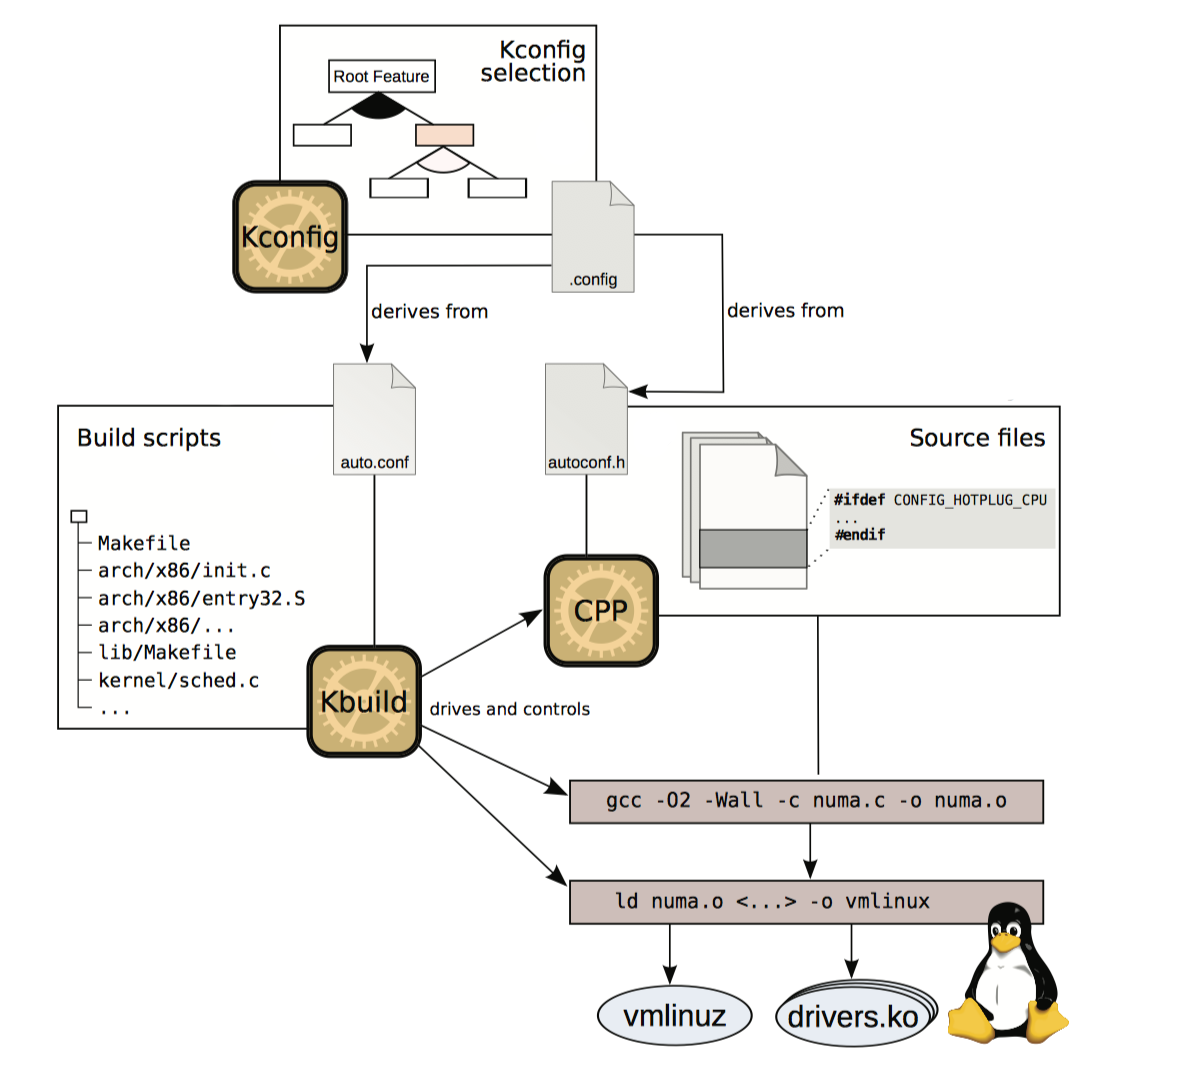
\includegraphics[width=1\textwidth]{img/linux-build2.png}
  \end{minipage}
\end{figure}

\autoref{linux-build} shows an overview over the Linux Kernel build process. The Linux build system relies on the KConfig system, Kbuild system and the C-Preprocessor to implement variability within the Linux Kernel product line. KConfig files  define configurable options while the Kbuild files specify the build process. A concrete and valid configuration can be genererated by leveraging the information within KConfig files. The creation of such an configuration can be achieved through user interfaces that aid in the configuration process. The result is a \texttt{.config} file that represents a concrete configuration. The build process itself is fully automated. Using the \texttt{.config} file, the files \texttt{auto.conf} and \texttt{autoconf.h} are generated. Those files are used during the build process to translate the concrete configuration into a compiled product. The result is a compiled and executable linux variant (\texttt{vmlinux}) together with dynamically loadable modules (\texttt{drivers.ko})

The KConfig system uses the KConfig language to specify available configuration options and dependencies among them \cite{variabilitymodel-linux}. Thereby the KConfig files define the variability model of the Linux Kernel. In contrast to the example we used in Section \ref{spl} to introduce variability models, the variability model of Linux is a decision model and not a feature model. However for simplification purposes, we will modify and extend the variability model shown in \autoref{featuremodel} in Section \ref{spl} to explain how variability is implemented within of the Linux Kernel. 

\begin{lstlisting}[caption= KConfig Language, label=kconfig]{language=KConfig}
config NETWORK_AUTHENTICATION
	bool "Network Authentication"
	depends on USER_AUTHENTICATION
	select NETWORK_SUPPORT
	select REMOTE_USER_FOLDER_SUPPORT if NETWORK_STORAGE_SUPPORT
	default y
	help
	  Support for network authentication ...
\end{lstlisting}
 
Building on top of the example shown in \autoref{featuremodel}, \autoref{kconfig} shows how the KConfig language can be used to describe the variability model. The example uses a Boolean variable that allows for either inclusion or exclusion of a feature in the configured product.
In the example, \texttt{NETWORK\_\-AUTHENTICATION} can only be selected if \texttt{USER\_\-AUTHENTICATION} has also been selected as \texttt{NETWORK\_\-AUTHENTICATION} depends on this feature. \texttt{If NETWORK\_\-AUTHENTICATION} is selected for inclusion in the compiled product, the features prefaced with \texttt{select} are automatically included aswell. It is also possible to define more complex conditions for \texttt{select} or \texttt{depends on} entries where the selection of a feature depends on more than one feature. In this instance \texttt{REMOTE\-\_USER\_\-FOLDER\_\-SUPPORT} is automatically selected if the \texttt{NETWORK\_\-STORAGE\-\_SUPPORT} feature is also configured to be included. Finally, \texttt{help} defines a text to provide the configuring user with information about the feature. This text is used in user interfaces for configuring the Linux Kernel such as menuconfig or xconfig.

 KConfig also offers an alternative option for including or excluding a feature: Tristate variables allow a feature to either be excluded, linked into the kernel statically, or be dynamically loadable \cite{variabilitymodel-linux}. Therefore the KConfig language allows the definition of the binding time for a certain feature. Other types of variables used in the KConfig language are integer and string.

The Kbuild build system uses the \texttt{auto.make} file together with other Kbuild Makefiles to define which sourcefiles to include for compilation. Because the Kbuild Makefiles define the build process of the product line, they represent the build model. Kbuild works by recursively processing the Makefiles within the directories and subdirectories of the Linux Kernel codebase to create two distinct lists containing objects that are to be included for the compilation process. The list obj-y contains all files that are to be compiled and linked whereas  obj-m contains those that will be compiled as loadable modules \cite{nadi-linux-kernel}\cite{makefiles.txt}. 

Finally \texttt{autoconf.h} defines variables for each selected KConfig feature \cite{Tartler:2011:FCC:1966445.1966451}. Defined variables within \texttt{autoconf.h} are used to evaluate compiler directives for including or excluding code sequences. All variables prefixed with \texttt{CONFIG\_} are variability variables originating from the KConfig system. \autoref{conditional-compilation} shows an examplary excerpt of source code. Lets assume that \texttt{autoconf.h} contained the line \texttt{\#define CONFIG\_\-NETWORK\_\-SUPPORT}. Because \texttt{CONFIG\_\-NETWORK\_\-SUPPORT} is defined, the \texttt{\#ifdef} statement within line 1 in our example evaluates to \texttt{true} and therefore the line \texttt{return 0;} is included for compilation of the  linux variant. If \texttt{CONFIG\_\-NETWORK\_\-SUPPORT} is not defined, \texttt{return 1;} gets included instad.

\begin{lstlisting}[caption=Conditional Compilation within the Linux Kernel, label=conditional-compilation]{language=C}
 # ifdef CONFIG_NETWORK_SUPPORT
   # return 0;
 # else 
   # return 1;
 # endif
\end{lstlisting}

For performing analyses on software product lines, the variability information within the Linux Kernel codebase can be extracted to create data models. The variability information within source files is translated into a code model while KConfig files can be used to create a variability model. Finally the Kbuild files define the build model of the Linux Kernel. After obtaining the models, they can be used to perform analyses on the software product line.

\subsection{Software Product Line Analyses}

This section will provide an overview of analyses that are tailored towards software product lines. We will later use the dead code analysis that will be introduced in Section \ref{feature-code-mapping}  for implementing an incremental analysis.

Measuring of relevant parameters (e.g. performance), testing and analyzing products is well established for individual products \cite[p.243]{Apel:2013:FSP:2541773}. 
In order to apply those methods on a the product line, a simple approach would be to analyze every possible permutation of feature combinations that is possible as a single product using the same established methods. For a product line with 33 independently selectable features and an analysis time of one second per permutation this would however result in an insurmountable computational effort of more than 272 years \cite{Thum:2014:CSA:2620784.2580950}. 

An approach that tries to handle this problem is to reduce the number of analyzed products thereby only covering a certain part of possible configurations rather than analyzing every single product. However this still results in analyses targeting single products instead of directly incorporating variability. 

In constrast to such \emph{product based analyses}, \emph{family based analyses} try to directly incorporate variability information within the analysis. In the following three sections, we will cover three categories of analyses incorporating variability that can be used to work with software product lines, ranging from analyses based on the feature model alone  to analyses processing statements and function calls. The categorization is based on the work of Apel et al.\cite{Apel:2013:FSP:2541773}.

\subsubsection{Feature Model Analyses}

We introduced the feature model as a way to describe variability within the Product Line in Section \ref{spl}. Using the information of the variabilty model, we can check for valid configurations and determine which features are mandatory.
Furthermore, features which can never be selected in a valid configuration can be identified and check the equivalency of two variability models.

As outlined in Section \ref{spl} and shown through examplary variability definitions using the KConfig language in Section \ref{linux-kernel}, the selection of features depends on constraints which are represented within the variability model. The constraints can be translated into logical formulas that allow to analyze different aspects of feature selection within the model.

Using the variability model of our operating system as shown in \autoref{featuremodel} as an example, making \texttt{NETWORK\_AUTHENTICATION} mandatory would also result in \texttt{NETWORK\_SUPPORT} becoming a mandatory feature as the authentication depends on it eventhough it is modelled as a mandatory feature.  According to Apel et al. \cite{Apel:2013:FSP:2541773}, other examples for feature model analyses include the detection of features that can never be selected or the examination of a given configuration to determine whether it is valid according to the feature model.

\subsubsection{Feature-To-Code-Mapping Analyses}\label{feature-code-mapping}

Feature-To-Code-Mapping Analyses use information about how selected configuration options are translated into compiled products. This means that those analyses may combine information from the variabiliy model with information from build or code model to compute their results.

An example of such an analysis is the \textbf{dead code analysis} as performed by the Undertaker tool \cite{Tartler:2011:FCC:1966445.1966451}. Undertaker uses configuration constraints within the variability model in combination with the code model to find dead or undead code segments. A dead code segment consists of code that will never be included in any valid configuration. An undead code segment on the other hand is a segment that will always be included for any valid configuration. Following up on the original work done by  Tartler et al. \cite{Tartler:2011:FCC:1966445.1966451}, Nadi and Holt also incorporated the build model into the dead code analysis \cite{mining-kbuild}. Undertaker creates a code model of the Linux Kernel consisting of codeblocks which are defined by \texttt{\#ifdef} directives. We will refer to analyses working based on such codeblocks as a \textbf{block based analyses}.

\autoref{dead-code} shows an example for dead code. As \texttt{CONFIG\_NETWORK\_SUPPORT} is automatically selected when \texttt{CONFIG\_NETWORK\_AUTHENTICATION} is selected, the conditions under which the encapsuled statement gets included for compilation can never be met. 

\begin{lstlisting}[caption=Dead Code, label=dead-code]{language=C}
 # ifdef CONFIG_NETWORK_AUTHENTICATION
   # ifdef !CONFIG_NETWORK_SUPPORT
     # printf("You can not sign in");
   # endif
 # endif
\end{lstlisting}

A condition that defines whether source code is included for compilation is called \emph{presence condition}. Through incorporation of the build model in the analysis, presence conditions can not only be extracted for blocks of code but also for source files. Let us assume a build model that excludes all source files related to network components during the build process when \texttt{NETWORK\_SUPPORT} was deselected during configuration. In this instance, any block within those files containing \texttt{\#ifdef !CONFIG\_NETWORK\_SUPPORT} would be considered a dead code block. Within the dead code analysis, SAT solving is used to determine whether the constraints for including a codeblock can be fulfilled. As SAT is NP-hard, this process requires a considerable computational effort.

\subsubsection{Variabilty-Aware Analyses}

A variability-aware analysis covers artifacts of the software product line without analyzing products individually \cite[p.261]{Apel:2013:FSP:2541773}. It aims to generate a result that allows to draw conclusions for individual configurations. In contrast to feature-code-mapping analyses, Variability-Aware analyses also incorporate effects of statements and function calls within the analysis.

Typechef is an example for a Variability-Aware Analysis that performs type checking on software product lines \cite{Dietrich:2012:RAV:2362536.2362544}. Type checking can be used to identify type errors like dangling method references and duplicate class names \cite{Thum:2014:CSA:2620784.2580950}. Typically the compiler checks for type errors when compiling a single product.  Variability-aware  checking helps to ensure that all variants of a product line are well typed without having to compile each variant \cite{Kenner:2010:TTT:1868688.1868693}. Typechef however requires more information than Undertaker within the code model and therefore uses a variability-aware parser for C-code that builds an abstract syntax tree which is then used to perform the analysis.

While the computations for variability-aware analyses are usually more costly than their counterparts for individual products, they do perform faster than product based analyses for product lines.

\subsection{KernelHaven - An Analysis Infrastructure}\label{kernelhaven}

KernelHaven is a an infrastructure for variability-based analyses of C-preprocessor software product lines such as the Linux Kernel \cite{KroeherEl-SharkawySchmid18}. It was initially created as a student project and is written in Java.  Since then, KernelHaven has been further developed and extended through numerous plugins. This section  provides an overview over the overall concept and features of KernelHaven and then describes the possibilites of extending KernelHaven through plugins. KernelHaven and its plugin infrastructure constitute the foundation for the system developed for incremental analyses that is described in Section \ref{implementation}. 

An overview over the KernelHaven architecture is shown in \autoref{pipeline}. Because KernelHaven targets C-Preprocessor based software product lines, it needs to be able to process build, variability and code model. KernelHaven achieves this by using extractors that extract data models from a given codebase. The analysis itself is then executed based on the extracted models. Extractors and analyses are configured as a pipeline through the Pipeline Configurator which uses a configuration-file to define the settings for the execution of KernelHaven. This configuration-file is translated into a configuration-object that then gets passed to each component of the pipeline by the PipelineConfigurator. It is  important to note that KernelHaven-plugins do not read their settings directly from a configuration file. This implementation will become relevant later as KernelHaven offers entry points to perform adjustments to the configuration read from the file.

\begin{figure}[h] 
  \centering
  \begin{minipage}[b]{1\textwidth} 
    \caption[KernelHaven-Pipeline]{KernelHaven-Architecture \cite{KroeherEl-SharkawySchmid18}}\label{pipeline}
    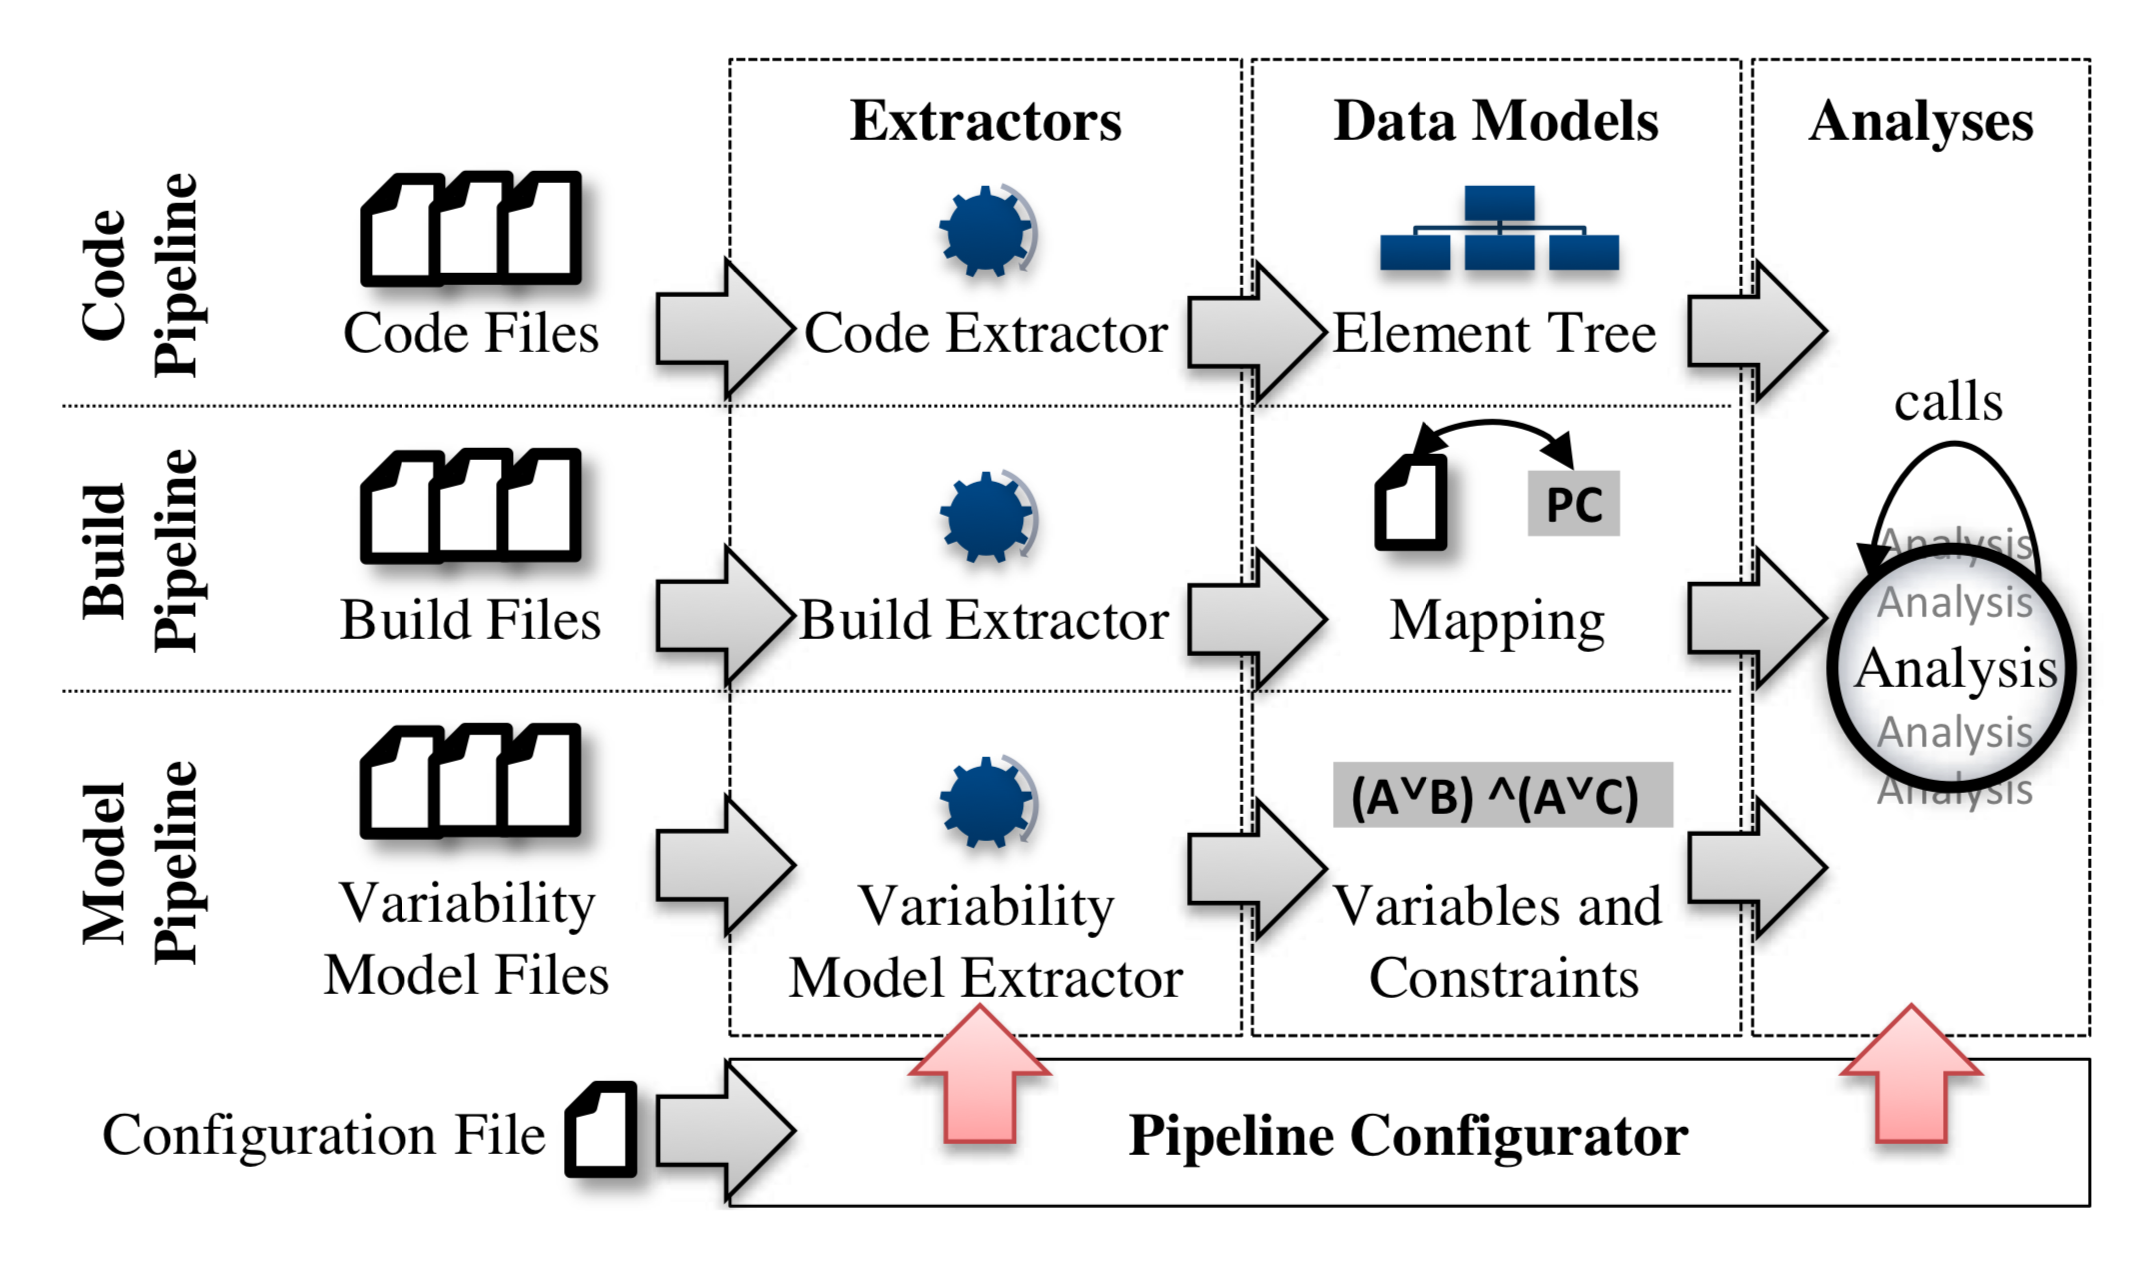
\includegraphics[width=1\textwidth]{img/KernelHaven-Pipeline.png}
  \end{minipage}
\end{figure}

By using a custom configuration-file, the user is able to configure existing Extractors and Analyses to suit his needs. However KernelHaven is also meant to be easily extendeable for developers and and therefore provides the possibility to extend the infrastructure through plugins.

KernelHaven can be extended through three types of plugins:

\begin{enumerate}
    \item Preparation-Plugins
	\item Extractor-Plugins
	\item Analysis-Plugins
	\item Utility-Plugins
\end{enumerate}

All of the plugins do not require adjustments to the main KernelHaven infrastructure but instead can be loaded as jar-files and automatically get added to the classpath when KernelHaven is started. Utility plugins do not really satisfy any plugin-interface of KernelHaven but contain components that are used by implementations of other plugin types. They must however still be loaded when KernelHaven is started as their components need to be accessible at runtime.

A Preparation-Plugin can define tasks that get executed before the KernelHaven-Pipeline is started. This can for example be useful for preprocessing inputs. Furthermore a PreparationPlugins allows to apply modifications to the configuration-object before the object is used by Extractor or Analysis-Plugins. However if no tasks need to be performed prior to the execution of the pipeline, no Preparation-Plugin needs to be defined for execution. 

Extractor-Plugins on the other hand are required to generate the models that the analysis can run on. There are three types of extractors: code model extractors, variability model extractors and build model extractors. Different extractors may work based on different files within the codebase. Furthermore the results of two different extractors for the same type of model may vary even if the same codebase was analyzed. This becomes clear when looking at two of the existing extractors for the code model. The TypeChef-Extractor based on the TypeChef-tool \cite{Kenner:2010:TTT:1868688.1868693} extracts a complete abstract syntax tree and uses macro expansion during the extraction of models from *.c files. The UndertakerExtractor based on the Undertaker-tool \cite{Tartler:2011:FCC:1966445.1966451} generates a representation of structure of \texttt{\#ifdef}-blocks.

While the KernelHaven infrastructure benefits from a selection of various extractors for the code model of the Linux Kernel, currently only one extractor is publically available for the build and another for the variability model of the Linux Kernel \footnote{\url{https://github.com/KernelHaven/KernelHaven/blob/master/README.md}}. The build model can be extracted using the KconfigReaderExtractor based on the KConfigReader-tool \cite{ck-kconfig} while the code model can be extracted through the KBuildMinerExtractor using the KbuildMiner-tool \cite{ck-kbuild}.

Both the KbuildMinerExtractor and the KconfigReaderExtractor are only able to extract the complete model represented through the codebase. This is not the case for the code model extractors which may also be configured to only process a subset of the files within the codebase. This is because the code model extractor is able to individually process each source file. Through header-files, extractors like the TypeChefExtractor might also consider other files when parsing one source file. Nevertheless an individual model for each source file is generated. This is not the case for KBuild and KConfig files as the KBuild and KConfig system both process complex dependencies that are spread between multiple files. Therefore the build- and variablity model are built viewing the information from all KConfig and KBuild files in total and not by looking at one individual file at a time.

Extractors may be configured to write extracted models to a cache-directory in order to reuse them for subsequent extectutions of KernelHaven removing the need to extract them again. Therefore KernelHaven does not necessarily require extractors to run for each execution of KernelHaven if the models already have been extracted before.

Finally Analysis-Plugins define the analysis that uses the extracted models. In order to ease the implementation of Analysis-Plugins, the plugins themselves do not have to take care of where the models come from. An analysis simply defines which models it needs and the corresponding extractors get started accordingly. This lets an analysis-developer focus directly on the work with the models themselves. Initially KernelHaven Analysis-Plugins  were single components that always processed the models directly. While the option to implement such an Analysis-Plugin still exists, KernelHaven also offeres the possiblity to implement AnalysisComponents that can be reused and combined to run after each other. An analysis that consits of such components is called a PipelineAnalysis. A PipelineAnalysis allows the results of one AnalysisComponent to be processed by the next one.  However only one type of result may be passed on to the next AnalysisComponent. In order to provide a simple means of rearranging and recombining analysis components, a custom domain specific language is implemented in KernelHaven allowing to define chains of AnalysisComponents from within the configuration-file itself thereby creating a PipelinaAnalysis. AnalysisComponents may also be combined through java-code which allows to cover corner cases that the domain specific language does not cover. A PipelineAnalysis implemented through java-code for example allows to still use the same AnalysisComponents in situations where  AnalysisComponents need to pass their output to multiple other components or AnalyisComponents need to pass on multiple types of results.

The KernelHaven readme file\footnote{\url{https://github.com/KernelHaven/KernelHaven/blob/master/README.md}} offers an overview over existing plugins. Later in this work, we will rely on exsiting AnalysisComponents within the UndeadAnalyzer-Plugin\footnote{\url{https://github.com/KernelHaven/UnDeadAnalyzer}} to implement an incremental dead code analysis. 

\newpage
\section{Requirements for the Implementation} \label{requirements}

This section lists the requirements for the implementation of a software system that enables incremental analyses. The developed system consists of an infrastructure for incremental analyses based on KernelHaven as well as an concrete implementation of an incremental dead code analysis for this infrastructure.

The information on each requirement broken down to four fields:

\begin{description}
    \item [Priority]
	This describes the priority of a requirement. The priority is given through the keywords Must, Should and May. The usage of the definitions takes RFC 2119 \cite{RFC-bum} as a guideline. Therefore \textbf{Must} describes a requirement that has to be implemented. \textbf{Should} indicates that the implemenentation of the requirement is strongly desired. Not fulfilling a Should requirement  does however still result in an acceptable overall system if the Must requirements are met. Finally \textbf{May} indicates a truely optional requirement. Those requirements represent additions to the system that are considered useful but at the same time are not valued as high as Must or Should requirements.
    \item [Source]
    The Source-field describes the origin of the requirement. Interview indicates that the source of information was the interview with my supervisor. Initial description indicates that the source of the requirements was the written description of the thesis goal as provided through my supervisor.
    \item [Description]
    this field provides a description of the requirement.
    \item [Explanation]
    Explanation provides further deatail on the requirement and may additionally provide reasoning as to why the requriement is included.
\end{description}

\begin{req}[Working Base of an Incremental Analysis] \label{req:working-base}
	\reqtable
	{Must}  {Interview}
	{The incremental infrastructure must allow analyses to work based on the current state of a repository and a proposed change.}
	{The working base of each incremental analysis is the previous state before a commit/code change. The increment is represented by the change introduced.}
	
	\begin{subreq}[Input Format for an Incremental Analysis] \label{req:git-diff}
		\reqtable
		{Must}  {Interview}
		{The incremental infrastructure must be able to process a git-diff file as input.}
		{The main input for the analysis is a git-diff file. This diff represents a changeset that is to be analysed.}
	\end{subreq}
\end{req}

\begin{req}[Covered Analysis-Types]\label{req:analysis-types}
	\reqtable
	{Must}  {Initial Description, Interview}
	{The incremental infrastructure must support block-based analyses. }
	{}
	
\end{req}


\begin{req}[Filtering of Extractor Input] \label{req:early-filtering}
\reqtable
	{Must}  {Interview}
	{The incremental infrastructure must allow the reduction of the set of files within the codebase upon which the extractors operate before files are processed by the extractors.}
	{Because extraction is costly, the filtering of artifacts must happen before the extractors are called.}
\end{req}

\begin{req}[Processing of Partial Models] \label{req:partial-models}
\reqtable
	{Must}  {Interview}
	{The incremental infrastructure must provide means for Analysis-Plugins to process parts of a model.}
	{In order to reduce the execution time of an analysis as described in Section \ref{concept}, mechansims need to be implemented that allow it to process partial models.}
\end{req}


\clearpage
\begin{req}[Configuration of Filters] \label{req:optimization}
\reqtable
	{Must}  {Initial Description}
	{
	The implemented infrastructure must provide means to configure different filters for processing the input.
    }
	{Depending on the extractor in use and the way it processes input files, different options cover different use cases. Furthermore different filters may affect the overall performance of the software system.}

\begin{subreq}[Implementation of Filters for Input]\label{req:mandatory-filters}
    \reqtable
	{Must}  {Interview, initial description}
	{
	The incremental infrastructure must at least include the filter options listed below (see REQ \ref{req:optimization}):
	\begin{itemize}
		\item \texttt{off} \\
		no filtering 
	    \item \texttt{change only} \\
	    only work with files that were modified
	    \item \texttt{variability-change only} \\
	     only work with files where the variability information was changed
	\end{itemize}
    }
	{In order to evaluate different filter methods and their effect on performance, different categories of filtering are required. \texttt{off} represents the state where no filtering is done, while \texttt{change only} performs superficial filtering without regarding variability information directly. Finally \texttt{variability-change only} is the most sophisticated filtering option of the three as it requires an analysis of the filecontent of each artifact itself.}
\end{subreq}

\begin{subreq}[Implementation of Effect-Filters] \label{req:effect-filters}
    \reqtable
	{May}  {Interview, initial description}
	{
	The incremental infrastructure may include the filter options listed below (see REQ \ref{req:optimization}):
	\begin{itemize}
		\item \texttt{change-effect} \\
		work with files that were modified and files that were indirectly affected by the change (eg. through includes)
	    \item \texttt{variability-effect}  \\
	    work with files where the variability information was changed and files that were indirectly affected by the variability change
	\end{itemize}
    }
	{When a file is modified, it may affect other files as well that were not changed directly. Depending on the extractors and analyses used it may be necessary to analyze those files as well.}
\end{subreq}

\end{req}

\begin{req}[Rollback must be possible] \label{req:rollback}
\reqtable
	{Must}  {Interview}
	{The incremental infrastructure must provide the option to revert back to the previous state after execution of an incremental analysis.}
	{An Analysis may change the source-files used as input for the extractors along with other changes. Those changes reflect the changes introduced by the new increment that was used as input. If that increment however contains defects identified by the analysis the user might choose to revert the changes and propose an alternative change. This alternative change can only be analyzed if KernelHaven reverts to the original state before the initial change.}

\end{req}

\begin{req}[Incremental dead code analysis] \label{req:dead-code-analysis}
\reqtable
	{Must}  {Initial Description}
	{An incremental dead code analysis must be implemented}
	{The dead code analyis serves as a practical example for block based analyses. It is used to demonstrate and evaluate the effectiveness of the incremental approach.}
	
	\begin{subreq}[Incremental dead code analysis Result Format] \label{req:format}
    \reqtable
    {Must}  {Interview}
	{The dead code analysis must provide a result in the same csv-format as implemented in the existing UnDeadAnalyzer\footnote{\url{https://github.com/KernelHaven/UnDeadAnalyzer}} plugin for Kernelhaven.}
	{Maintaining the same format as the non-incremental dead code analysis allows for comparability between incremental and non-incremental analyses. \\
	\emph{Note: eventhough the csv-format remains unchangend, the contents of incremental and non-incremental result-files might differ (see REQ \ref{req:coverage})}}
	\end{subreq}
	
	\begin{subreq}[Incremental dead code analysis Result Coverage] \label{req:coverage}
    \reqtable
    {Must}  {Interview, Feedback from Presentation of Initial Concept}
	{The dead code analysis should produce a result that only contains dead code blocks that were found during the latest analysis executions.}
	{As the analysis should provide feedback for the developer on his work, parts of the software system which could not have been affected by the changes he introduced do not need to be represented in the result. Therefore merging the result of the increment with previous results is not desired.}
	\end{subreq}
\end{req}

\clearpage
\begin{req}[Target Artifacts] \label{req:target-artifacts}
\reqtable
    {Must}  {Initial Description}
	{The incremental infrastructure must support the processing of *.c, *.h, makefile, Kbuild and Kconfig files}
	{The filetypes listed above represent the code, build and variability model of the Linux Kernel. As the Linux Kernel is used for the evaluation of the implemented incremental analysis approach, those filetypes need to be considered.}
\end{req}


\begin{req}[Run existing KernelHaven-Analyses incrementally] \label{req:existing-analyses}
\reqtable
    {Should}  {Interview \\ \emph{Note: This requirement emerged after the implementation choice to use the KernelHaven infrastructure was made}}
	{The incremental infrastructure should enable reuse of existing AnalysisCompontents .}
	{Existing analysis plugins for KernelHaven have been written as non-incremental analyses. The adaptation of existing analyses removes the need to reimplement existing analyses. Furthermore the adaptation of existing plugins allows for a performance evaluation of incremental analyses against non-incremental analyses.}
\end{req}

\newpage

\section{Concept for Incremental Analyses}\label{concept}

KernelHaven and other software tools such as Undertaker\cite{Tartler:2011:FCC:1966445.1966451} currently allow to analyze a given codebase in its entirety. When changes to the codebase are introduced, the entire codebase must be analyzed again resulting in costly computations. This is because the model-extraction has to be redone and the subsequent analysis has to redo the computation for the new models. Assuming that an analysis consists of model-extraction and subsequent computations based on the extracted models, we are presented with two options to reduce computational effort:

\begin{enumerate}
	\item Reduction of computational effort for the extractors \\
	\emph{Extraction does not need to happen on the entire codebase - only the parts that changed dictate what to extract}
	\item Reduction of computational effort for the analysis performed on the extracted models \\
	\emph{Models do not need to be processed again completely - only the parts that changed dictate what to process}
\end{enumerate}

We refer to an analysis that utilizes one or both of those measures to reduce the computational effort when changes are introduced as an incremental analysis.

The first option can be achieved by the filtering of input files so that only files that were affected by changes need to be extracted. The most trivial possibility to reduce effort is to define that where a file was left unmodified, no new extraction needs to happen. 
However a file change does not necessarily result in changed variability information - and as models are extracted to obtain variability information, files where that information did not change can also be excluded. Filtering files based on changed variability further reduces the computational effort for obtaining the models. Filtering based on file and variability changes within single files can be used when every file is handled isolated from other files within the extraction logic.

While the described approach certainly makes sense for some scenarios, it does not suffice for others. If a file changes, it might affect the models of another file aswell if dependencies exist between those two files. Depending on whether or not the extraction logic includes those dependencies when building a model for a single file, different models might be computed for the same file even if the file itself is unchanged. An example for this is the extraction logic of TypeChef \cite{Kenner:2010:TTT:1868688.1868693}. Typechef uses macro expansion to compute the models for each sourcefile and thereby includes information from other files. 

Therefore filtering for direct file changes or variability changes within a single file is not sufficient for every situation. Instead it might be necessary to also include files that have been affected by the change. In order to keep the concept for incremental analyses generic enough to cover those use cases, different filtering mechanism must be applicable (see REQ \ref{req:optimization}). However the extraction of a partial model is only possible if the extraction logic itself allows that. As already mentioned in Section \ref{kernelhaven}, the existing code model-extractors for KernelHaven  are able to run on a subset of files thereby extracting a partial model.  This is not the case for build model and variability model extractors. Therefore as soon as one of the related files changes, the entire model needs to be extracted.  

At the end of the extraction process, the complete code, build and variabilitymodel can be provided by merging the extracted parts with the models representing the previous state of the codebase. This allows the analysis to have full access to the models eventhough the computational effort was reduced for the extraction itself.

Now the second option can be applied. Depending on the analysis that is performed, it is possible that only a part of the models must be processed because the analysis-results for the other parts were unaffected by the changes to the codebase. The dead code analysis is an example for an analysis that is able to work based on a partial code model. The implementation of the dead code analysis is described in \autoref{incremental-dead-code-analysis}.


\clearpage


\section{Implementation of Incremental Analyses}\label{implementation}

This section describes the implementation of an infrastructure for incremental analyses and provides reasoning for the decisions made when engineering the infrastructure. The term \emph{incremental analyses} will henceforth be used as shorthand for incremental analyses that are block based as only those are targeteted by the implemented infrastructure (see REQ \ref{req:analysis-types}).

The infrastructure itself is based on KernelHaven \cite{KernelHaven} as KernelHaven together with its plugins provides a working implementation for various software product line analyses. Through KernelHaven's plugin interfaces, it is also possible to implement the infrastructure for incremental analyses as a plugin itself.

By extending an existing infrastructure like KernelHaven, we can benefit from an existing codebase as well as future developments within the KernelHaven project. Furthermore future users of the incremental infrastructure can adjust existing non-incremental analyses written for KernelHaven to run as incremental analyses.

\subsection{Two Phases of Non-Incremental Analyses}\label{2-phases}

The execution of an analysis in KernelHaven in most cases can be broken down into two mandatory phases as shown in \autoref{2-phases-image}. In the Extraction-Phase, KernelHaven extracts models from the codebase  (or alternatively reads them from the cache). In the Analysis-Phase, the resulting models are used to compute the analysis results.

\begin{figure}[h] 
  \centering
  \begin{minipage}[b]{1\textwidth} 
    \caption[Non-Incremental Analysis: Two Phases]{Non-Incremental Analysis: Two Phases}\label{2-phases-image}
    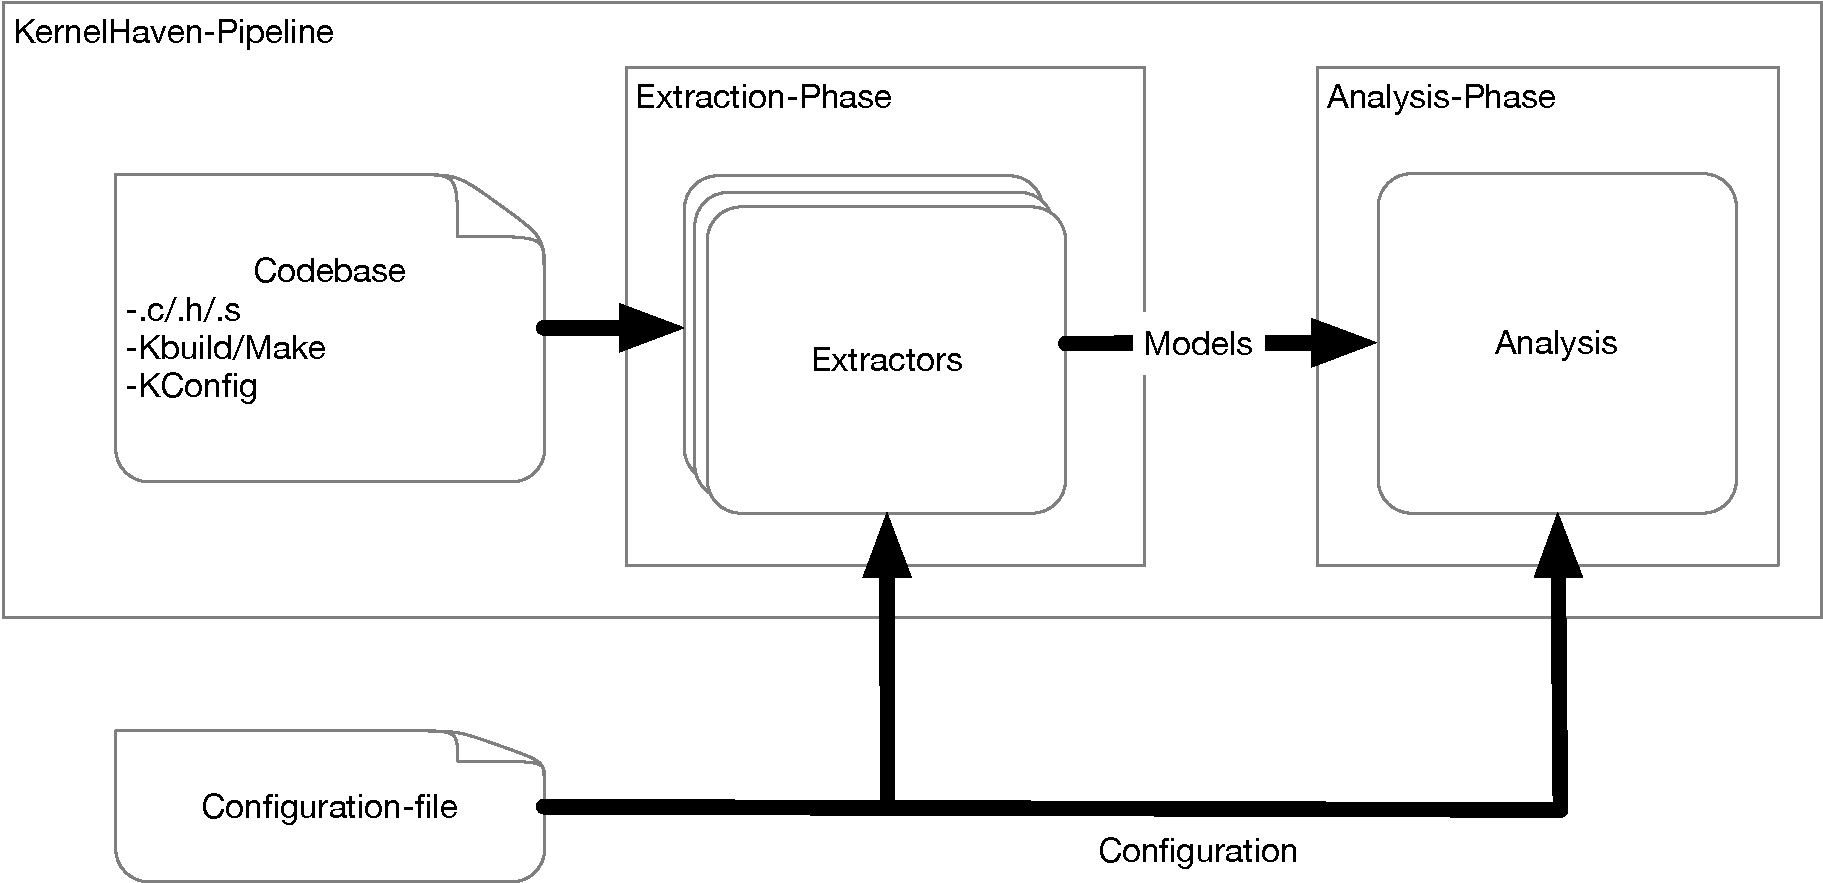
\includegraphics[width=1\textwidth]{img/KernelHaven.pdf}
  \end{minipage}
\end{figure}


While this view does ignore some technical aspects, it focuses on the core aspects of an analysis execution. Therefore it does not try to replicate the configuration mechanism of KernelHaven and instead only visualizes the configuration of the pipeline components as a direct result of the configuration file. This simplification makes it easier to understand the required modifications for performing incremental analyses. The required modifications for performing incremental analyses will be presented in the next section.

\subsection{Four Phases of an Incremental Analysis}

While the Analysis- and Extraction-Phase as described in \autoref{2-phases} are also present for analyses implemented with the incremental infrastructure, there are additional mandatory tasks which get executed in two more phases - the Preparation-Phase and the Post-Extraction-Phase. The resulting four phases are visualized in \autoref{4-phases}.

The Preparation-Phase is the first phase in an incremental analysis. Its purpose is to update the codebase and reduce the number of files that the extraction has to run on (see REQ \ref{req:early-filtering}). This saves computational effort when running the extractors as some parts of the codebase  may not need to be processed again. Instead the result of previous extractions may be reused. In fact some (or all) of the extractors might not even need to be executed at all if the files they work with did not change. For the code model, KernelHaven allows the configuration-object to define which files the extractor should run on. 
 Therefore the configuration is not simply read from the configuration-file and passed on without modification but instead gets modified to activate or deactivate extractors and to define the relevant subset of files for the code extractor. Those modifications happens in the Preparation-Phase before the Extraction-Phase starts.

 But even before any filtering on the artifacts in the codebase happens, the incremental infrastructure ensures that the codebase represents the increment that is to be analyzed. This is possible to achieve by using a git-diff file describing changes to the codebase (see REQ \ref{req:git-diff}). In order to allow for reuse of existing extractors, the changes need to be applied to the codebase on the filesystem. This is the extractor-plugins for KernelHaven work based on access to the filesystem and can not work with data streams.

Because of the filtering performed in the Preparation-Phase, the analysis may not simply run on the result of the extractors directly as the result is not neccessarily a complete representation of all three models. Therefore the result is merged with the results of previous extractions. After merging, it makes the resulting code-, build- and variabilitymodel available to the analysis through the \texttt{Hybrid\-Cache}.

While merging the extractors outputs, it is important that no prior extraction results get overwritten. This is because REQ \ref{req:rollback} requires that the state before the execution of an incremental analysis can be restored. Therefore the Post-Extraction-Phase uses a modified implementation of the cache-system, that the main infrastructure of KernelHaven uses. This \texttt{Hybrid\-Cache} allows storage and access to two versions of the code-, build- and variabilitymodel. It guarantees that the previous code-, build- and variabilitymodel can be restored.

While a rollback to previous extraction-results is the main reason for introducing the \texttt{Hybrid\-Cache}, a side benefit is that analyses now may use both the current and the previous state of the codebase. This could be relevant for future implementations of incremental analyses that draw benefits from comparing the old and the new model. It would for example be possible for analyses to identify changes based on the models directly instead of the task being handled in the Preparation-Phase. Consequently, it would be relativly easy to implement analyses offering similar optimizations as the \texttt{change-effect} option described in REQ \ref{req:effect-filters} by only performing analyses on changed parts of the models - the drawback being that the extractors would still need to process the entire codebase.

\clearpage
\begin{figure}[h] 
  \centering
  \begin{minipage}[b]{1\textwidth} 
    \caption[Incremental Analysis: Four Phases]{Incremental Analysis: Four Phases}\label{4-phases}
    \centering
    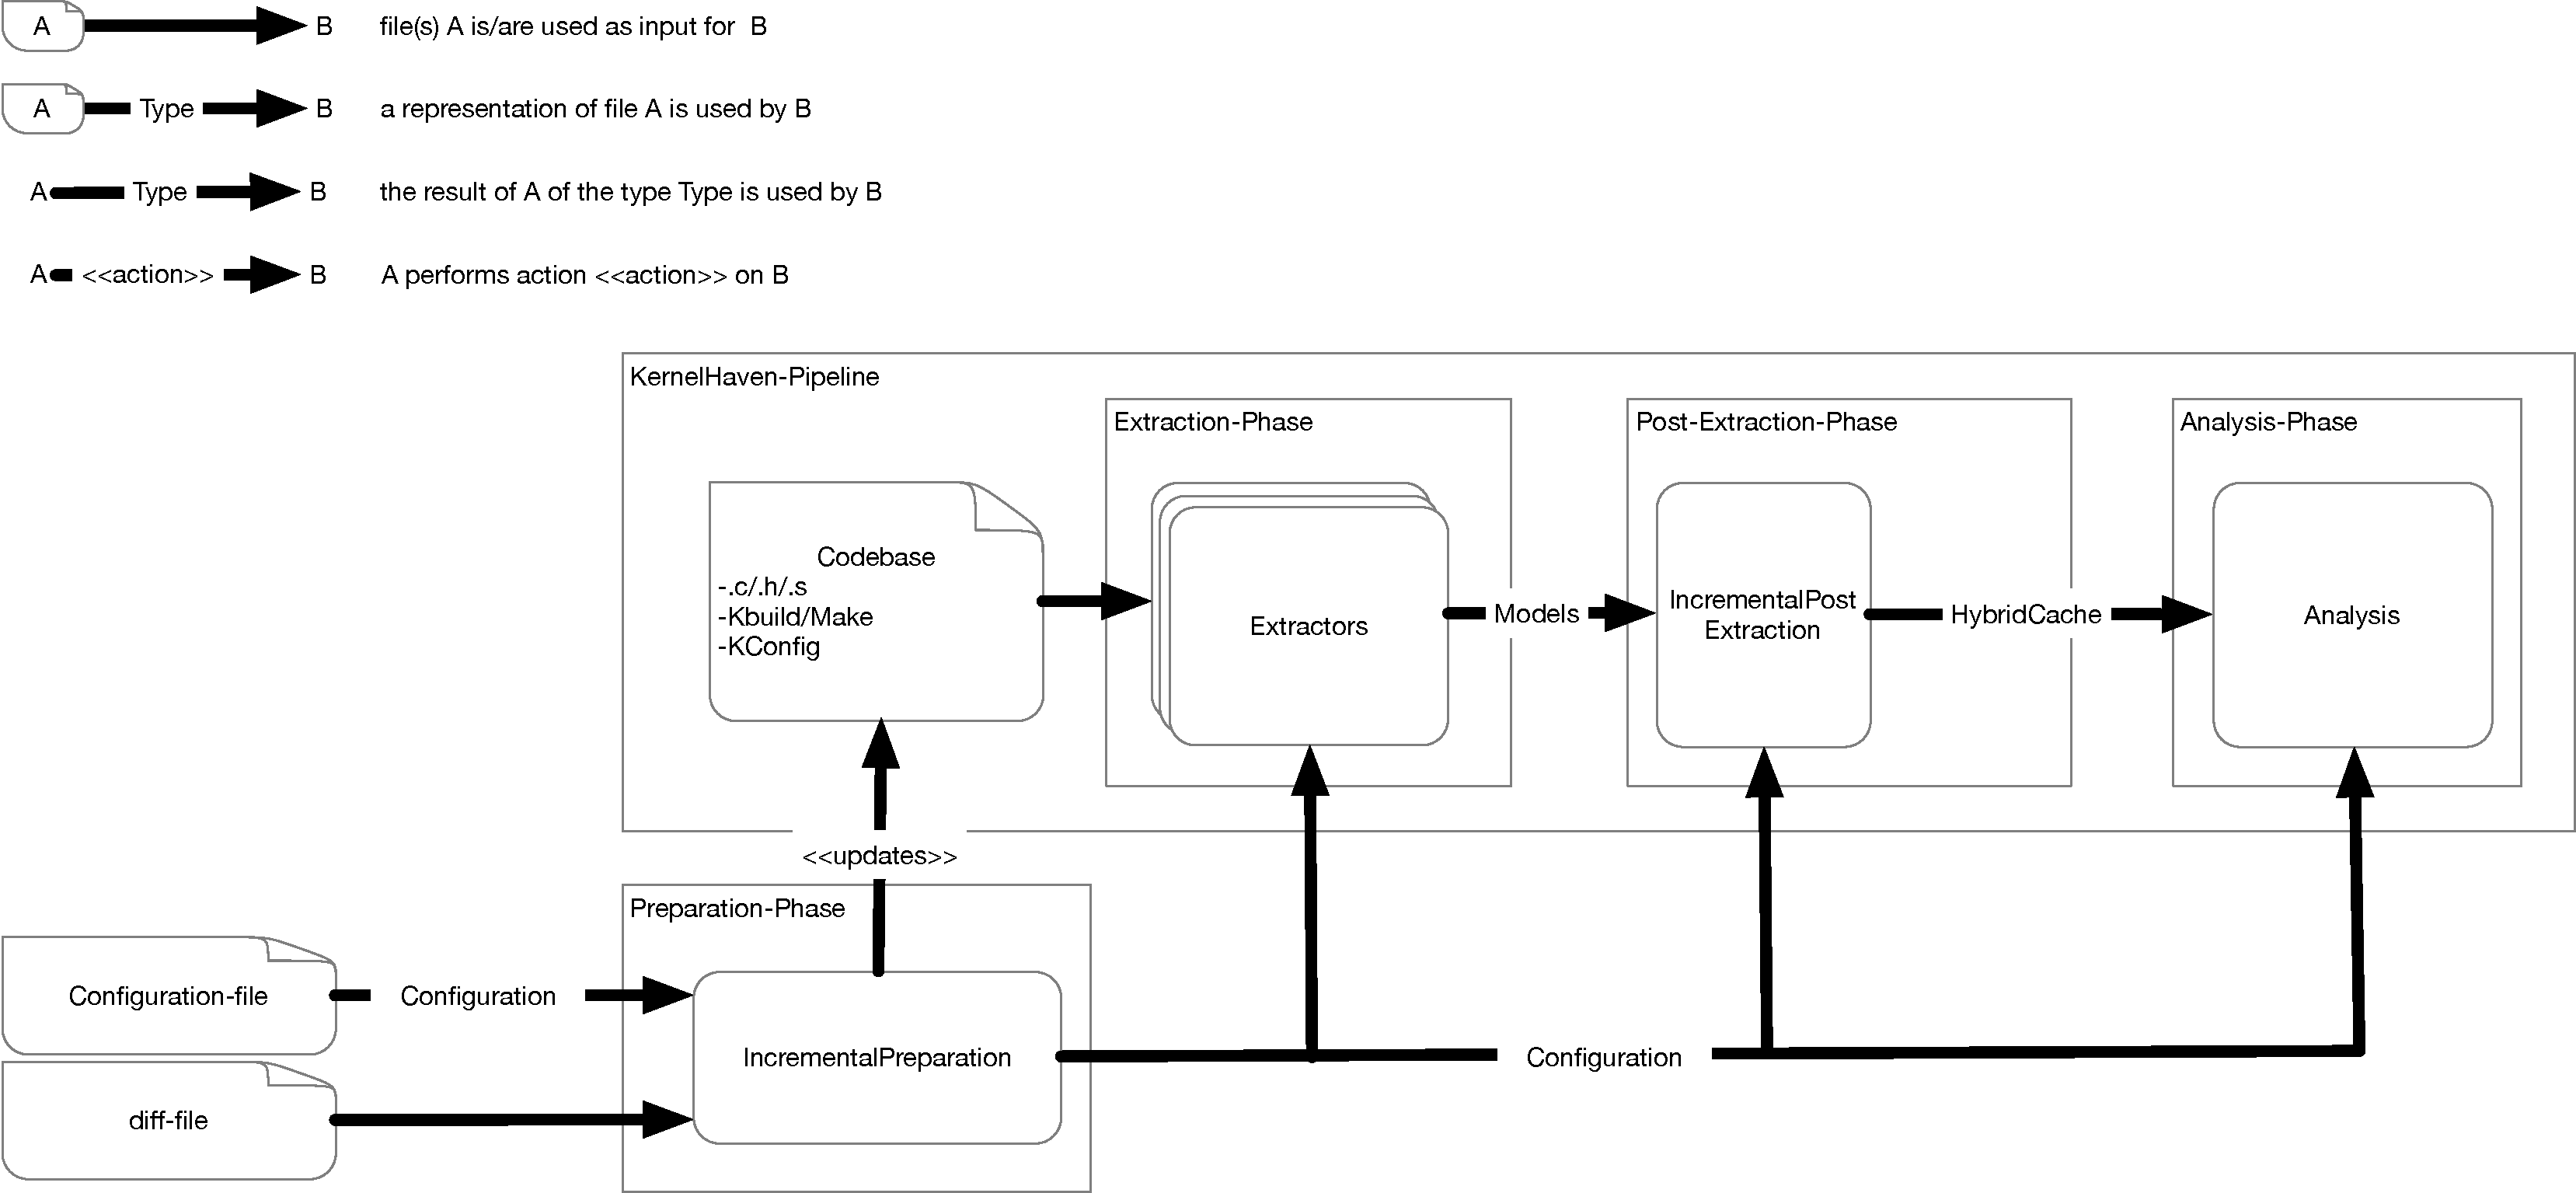
\includegraphics[width=0.9\textheight, angle=90]{img/KernelHavenIncremental.pdf}
  \end{minipage}
\end{figure}
\clearpage


\subsection{Implementation of the Preparation-Phase}\label{preparation-phase}

Because the definition of inputs for the extractors of the Preparation-Component needs to happen before the extraction and analysis itself, it makes sense to run them before an analysis is instantiated. In Section \ref{kernelhaven}, Preparation plugins were introduced as a means to execute tasks prior to the execution of the Analysis or Extractor plugins. We use the \texttt{IPrepraration}-interface to implement the tasks of the preparation phase.

An alternative to this approach would have been to configure extractors from within an analysis-plugin through the implementation of an \texttt{Analysis\-Component} or \texttt{PipelineAnalysis}. In this case, the analysis-plugin would have to care about the configuration of extractors and the content of the codebase on the filesystem. This is possible because KernelHaven is implemented as a pull-pipeline. The component at the very end of the pipeline could technically modify the way that prior components work. It would however represent a breach in the data-flow to have the last component modify the inputs and configuration for prior  components. 

In a non-incremental analysis, the definition of the configuration happens before the pipeline is started when writing the configuration-file. Some parameters of the configuration might get overwritten by command line parameters when the pipeline is set up by the \texttt{PipelineConfigurator}, the class responsible for putting all parts together before starting the pipeline - however the configuration is not directly modified from extractors or analyses. Using the \texttt{IPreparation}-interface preserves the data-flow within KernelHaven.

Furthermore, the \texttt{IPreparation}-interface offers more flexibility to adjust the configuration of KernelHaven as all parts of the infrastructure - even the actual analysis-class itself - can be configured from within an \texttt{IPreparation}-implementation. Therefore the modifiability of the incremental infrastructure is higher than with analysis-classes which may only change the configuration for extractors.

For the incremental infrastructure, the \texttt{Incremental\-Preparation}-class implements the \texttt{IPreparation}-interface and merges the changes described by the diff-file with the exisiting codebase. It then continues to filter the files within the codebase to reduce them to a subset that the extraction needs to run on. The configuration then is updated by defining the actual input-files upon which the extractors are run.

\subsubsection{Updating the Codebase}\label{git-apply}

The changes to the codebase are described through a git-diff file (see REQ \ref{req:git-diff}) . While it is technically possible to create own implementations that apply those changes to files on the filesystem, we use the \texttt{git apply} command. \texttt{git apply} allows to apply changes in git-diff file to a given directory even if that directory is not a git repository. All that is required is command line call from within the folder on which the command should be applied:

\begin{lstlisting}[language=bash]
  $ git apply path/to/git.diff
\end{lstlisting}

 Furthermore \texttt{git apply} also allows to revert changes thereby ensuring the fulfillment of REQ \ref{req:rollback}:
 \begin{lstlisting}[language=bash]
  $ git apply --reverse path/to/git.diff
\end{lstlisting}
 
 A downside to using \texttt{git apply} is that it requires git to be installed on the system that KernelHaven is executed on. However because we assume a git-diff file as input (see REQ \ref{req:git-diff}), it is reasonable to assume that git is most likely already installed on the executing system.

Furthermore there are several advantages to using \texttt{git apply}. As the input is defined by the creation of a git-diff file through the \texttt{git diff} command, also using git to apply the changes ensures compatibility with the file. Therefore we assume that the existing git implementation is less prone to errors than an own implementation or other third party implementations. The integration of \texttt{git apply} results in a low implementation effort as command line calls can easily be realized through the Java \texttt{ProcessBuilder}\footnote{ProcessBuilder documentation: \url{https://docs.oracle.com/javase/7/docs/api/java/lang/ProcessBuilder.html}}.

\subsubsection{Filtering of Files within the Codebase}\label{filtering-input}

After the codebase was updated, all files represeting variability within the revision that is to be analyzed are available for subsequent processing. To fulfill REQ \ref{req:early-filtering}, a filtering mechanism is implemented. Filters can be configured individually for code-, build-, and variability-files through the configuration-file.

One important resource that the filters use is an abstraction of the git-diff file that was used as input. This abstraction is implemented through the \texttt{DiffFile}-class.
An instance of the \texttt{DiffFile}-class contains an entry for each file that was affected by the changes described in the git-diff file that was used as input. For each entry, one of the following types of change is included:

\begin{itemize}
	\item \texttt{MODIFICATION} \\
	      indicates a modification of the file
	\item \texttt{ADDITION} \\
	      indicates the addition of the file
	\item \texttt{DELETION} \\
	      indicates the deletion of the file
\end{itemize}

Furthermore the entries contain information on whether the variability is changed through the according git-diff file. So each entry is assigned one of the following markers aswell:

\begin{itemize}
	\item \texttt{CHANGE} \\
	      indicates changed variability
	\item \texttt{NO\_CHANGE} \\
	      indicates unchanged variability
	\item \texttt{NOT\_A\_VARIABILITY\_FILE}\\
	      indicates that the file was not considered to be a filetype that carries variability information
	\item \texttt{NOT\_ANALYZED}\\
	      indicates that the entry for the file was not checked for variability changes
\end{itemize}

Creating an abstraction of the git-diff file requires that the file itself is read and interpreted. This is done by a \texttt{DiffAnalyzer}, a class that takes the git-diff file used as input and translates it into a \texttt{DiffFile}-object. There are two existing \texttt{DiffAnalyzer}s implemented within the incremental infrastructure: the \texttt{Simple\-Diff\-Analyzer} which only looks for the type of change without considering variability and the \texttt{Variability\-Diff\-Analyzer} which also analyses for variability changes. The advantage of the \texttt{Simple\-Diff\-Analyzer} is that it is faster than the \texttt{Variability\-Diff\-Analyzer}. For the largest git-diff file that we analyzed during evaluation as described in Section \ref{evaluation}, the \texttt{Simple\-Diff\-Analyzer} took approximately four seconds while the \texttt{Variability\-Diff\-Analyzer} took almost an hour. However those results reflect the processing on an 800MB sized commit describing the complete content of every file within the codebase. The long duration required for the \texttt{Variability\-Diff\-Analyzer} does not mean that introduces significant cost for every commit that is analyzed (as those are usually much smaller) but yet still shows that the \texttt{Simple\-Diff\-Analyzer} is able to process git-diff files much faster.
Therefore it makes sense to always use the \texttt{Simple\-Diff\-Analyzer} when variability-information is not needed for filtering. Because the \texttt{Simple\-Diff\-Analyzer} does not analyze for variability changes, every file entry that it processes will remain marked as \texttt{NOT\_ANALYZED}.

The \texttt{DiffFile}-object is generated before the filters are applied and then passed to them as input. The reason for not handling the interpretation of the git-diff file directly within the filters is that this would result in all three filters having to do the interpretation separately thereby creating computational overhead.

The implementation of \texttt{Variability\-Diff\-Analyzer} relies on previous work which performed a commit based analysis of software product line evolution \cite{ComAn}. The tool used and implemented for this analysis  is called ComAn \cite{ComAn-tool}. Because the paper covers commits to the Linux Kernel, the tool is able to process git-diff files describing changes within the codebase of the Linux Kernel. 

ComAn allows to extract the number of lines where variability information is modified for each changed file that is described in the git-diff file. This information is used within the \texttt{Variability\-Diff\-Analyzer} to determine which files contain variability changes. If one or more lines within the changes for a file modified variability information, the file is marked as \texttt{CHANGE}. Otherwise it is marked as \texttt{NO\_CHANGE} or \texttt{NOT\_A\_VARIABILITY\_FILE} depending on whether ComAn considers it to be a filetype that could be relevant for variability within the codebase. 

The result of the \texttt{DiffAnalyzer} (the \texttt{DiffFile}-object) then gets passed to the filters together with the path to the codebase on the filesystem and a regular expression describing which files to include. Those regular expressions can be configured individually for files related to the code, build and variability model through the configuration file. If they are not defined within the configuration file, default values will be used \footnote{refer to the following resource  for the default values: \url{https://github.com/KernelHaven/KernelHaven/blob/master/src/net/ssehub/kernel_haven/config/DefaultSettings.java}}. The regular expression for code files is also used directly by the code model extractors. It defines which types of files within the codebase the code model extractor runs on for both incremental and non-incrementel KernelHaven executions. The regular expressions for build and variability model are currently only used by the incremental infrastructure and do not influence any existing extractor directly. In the incremental infrastructure the regular expressions are used to determine which files within the codebase correspond to which model type. Therefore the regular expression used for each of the models is essential for correct filtering. If the expression does not match all the relevant files for one type of model, this may result in an incorrect extraction process and therefore inconsistent results.

The output of each filter is a list of all the paths that should be included for extraction. Because a separate filter is responsible for each type of model, three lists are created separately for the extractors for build-, variability and code model. As already mentioned in Section \ref{kernelhaven}, currently only extractors for the code model can handle running on a subset of files within the codebase. As a result, both build- and variabilitymodel need to be extracted from scratch based on the entire codebase as soon as at least one corresponding file with a variability change.

Each of the three separate filters for the code-, build- and variabilitymodel can be configured individually but in some cases one implementation can also be reused for all models. This is because the regular expression may allow sufficient adjustments for each model type. For example a filter that filters for file changes only can process each file in the same exact way no matter what it contains - however by providing a regular expression, it is able to return only files of a certain type. Therefore it is able to filter individually for files of the build, variability or code model.

 Any filter implementations must extend the abstract \texttt{InputFilter}-class. The following filters are included in the incremental infrastructure - all of which can be applied to code-, build- and variabilitymodel:

\begin{itemize}
\item \texttt{DefaultFilter} \\
    This filter lists all files within the directory of the codebase and filters them using the regular expression on the file-path. If all files representing the build, code or variability model within the codebase are matched by the regular expression, this filter represents the off option described in REQ \ref{req:optimization}. This is because it then matches all files within the codebase that the extractors can potentially process thereby resulting in a full extraction of every model.
\item \texttt{ChangeFilter} \\
    filters according to the change only option described in REQ \ref{req:optimization}. This filter takes the entries from the \texttt{DiffFile}-object where the file was either marked as \texttt{ADDITION} or \texttt{MODIFICATION} and then filters the file-paths for the regular expression. Furthermore the filter can be configured to also include \texttt{DELETION} entries.
\item \texttt{VariabilityChangeFilter} \\
    filters according to the variabilty change only option described in REQ \ref{req:optimization}. This filter filters similar\footnote{only considers entries marked as \texttt{ADDITION} or \texttt{MODIFICATION}, filters for regular expression, can be set to include \texttt{DELETION} entries} to the \texttt{ChangeFilter}  but reduces the set of files even further by only including the files where the variability was marked as \texttt{CHANGE}. It requires that the git-diff file was analyzed using the \texttt{Variability\-Diff\-Analyzer}.
\end{itemize}

Because each code file can be extracted separately, we can ignore \texttt{DELETION}-entries for when extracting the codemodel. Instead the \texttt{DELETION}-entries concerning the code model will be handled later when merging the models by simply deleting the parts of the model that represent files that were deleted. This is not the case for variabilty and build extractors as an extraction always covers the entire model. Because deleted files potentially modify the model and we do not have the option to simply remove deleted parts from models extracted in earlier iterations, \texttt{DELETION}-entries are also included in the filter result. Thereby  build and variability model extractors are also executed when the only changes to the respective files within the codebase are deletions.

\subsubsection{Modifying the Configuration}

Based on the results of the filters, the configuration is adjusted. If the list of paths is empty for the code, variability or build model, the corresponding extractor does not run as the previous model can simply be reused. To achieve this, the extractors are either turned off or switched on through a configuration option. The modifications to the configuration constitute the final step of the Preparation-Phase.

For the code model, extractors are able to run on a subset of files within the codebase. Therefore the extractor for the code model has a configuration-option to define which files are to be processed. Using this configuration option, the entire list of filtered elements is passed to the code model-extractor.


\subsection{Implementation of the Post-Extraction-Phase}\label{post-extraction-phase}

In the Post-Extraction-Phase, extraction results are merged with the models extracted in previous iterations and then provided to subsequent analyses. This is implemented in the \texttt{Incremental\-Post\-Extraction}-class. 
\texttt{Incremental\-Post\-Extraction} is written as an analysis plugin because it has a similar point of entry as an analysis: it expects results from the extractors results and processes them. As mentioned in Section \ref{kernelhaven}, there are two options for implementing an analysis plugin in KernelHaven - one is to implement a single analysis class and the other to implement an AnaylsisComponent that can be used in combination with other analysis components to consitute an analysis. AnalysisComponents are implemented by extending the \texttt{Analysis\-Component}-class. A component passes its result on to the next component which then works based on that input. The advantage of the using \texttt{Analysis\-Component} implementation is the possibility for reuse of software components. If multiple different analyses require the same step to be performed somewhere along the way, they can simply reuse the \texttt{Analysis\-Component} that performs that step.

For \texttt{Analysis\-Component}s KernelHaven assumes that those components are chained together and executed in the defined order. Not using \texttt{Analysis\-Component}s therefore might hold advantages when this strict pattern needs to be broken - for example by skipping steps or repeating a certain step depending on the result of a subsequent step.

However the tasks of the Post-Extraction-Phase are mandatory before the Analysis-Phase starts. Therefore reuse of the component that implements the tasks is of paramount importance. Consequently \texttt{Incremental\-Post\-Extraction} is written as an \texttt{Analysis\-Component}.

\subsubsection{Pulling Extractor Results}

\texttt{Incremental\-Post\-Extraction} can pull results from all three extractors in order to merge them with previously extracted models. \texttt{Incremental\-Preparation} defines whether new results for code, build and variablity model need to be extracted by modifying the configuration-object. Using the configuration-object, \texttt{Incremental\-Post\-Extraction} is able to selectively request the result of the code-, build or variabilitymodel-extractor. Therefore only the extractors where the model - or for the codmodel parts of the model - need to be extracted are started. It is important that the extractors only run when their results are used to prevent computational overhead.

However because of how KernelHaven handles the extraction of models, this required adjustments to the KernelHaven infrastructure. In KernelHaven, an analysis defines which models are needed through its constructor. KernelHaven assumes that it needs to provide all models required by the analysis to it through its extractors. Therefore KernelHaven starts the extractors even before the results of the extractors are requested from within the analysis. 

\texttt{Incremental\-Post\-Extraction} is implemented as an analysis-plugin that potentially requires results from all extractors but may end up requesting none of them. So while its constructor signals that all three models are required, this does not necessarily match the need to extract them. To overcome this obstacle, a configuration option was implemented in KernelHaven so that the extractor start is delayed until the result of the extractor is requested. While this configuration option may also be used from within the configuration-file for other analyses, it gets set automatically within \texttt{Incremental\-Preparation} as soon as not all three models need to be extracted.

An alternative to this approach would have been to provide multiple implementations for the Post-Extraction-Phase. As the extractors are started depending on the models defined in the constructor of the analysis, implementations similar to \texttt{Incremental\-Post\-Extraction} covering each combination of code, build and variabilitymodel would have been required. This would have resulted in additional clutter from the classes themselves. Furthermore \texttt{Incremental\-Post\-Extraction} would always need to reconfigure the configuration so that the Post-Extraction-Implementation in use matches the models that need to be extracted. While this has the advantage that no changes to the main KernelHaven infrastructure would be neccessary, this option was disregarded in order to keep the implementaition clutter-free and concise.

A third option would have been to introduce configuration-options to KernelHaven that directly block the extractors from running. While this is technically feasible, it does contradict the design of KernelHaven. The configured analysis in KernelHaven dictates which models it needs. Based on the requirements of the analysis, the KernelHaven infrastructure is then expected to deliver the required models.  Therefore blocking extractor executions hinders the KernelHaven infrastructure from fulfilling its designed purpose. 

\subsubsection{Merging Extractor Results}

Having access to the results of the current execution of the extractors is not enough as an analysis may need the complete models and only a subset of them might have been newly extracted. Therefore extracted models get stored for access in subsequent iterations of an incremental analysis. The very first execution of the incremental infrastructure extracts and stores the initial models while subsequent executions perform updates on the initially extracted models. However it is not sufficient to simply update the model - the previous version of the model must be accessible in order to allow a rollback as described in REQ \ref{req:rollback}. The storage of the current and previous version of the models is implemented in the \texttt{Hybrid\-Cache}.

\texttt{Hybrid\-Cache} itself uses the same caching-implementation that KernelHaven uses for its cache. This means that it works based on the filesystem and writes serialized models to a cache-folder. The variability and build model are represented by a single file while the code model is represented by multiple files - meaning that each sourcefile constituting the code model is represented by one file within \texttt{Hybrid\-Cache}.
 
 In contrast to KernelHavens cache however, the \texttt{Hybrid\-Cache} uses multiple folders to store its files. The core idea is to have one folder describing all current models called 'current' and another folder called 'history' describing the changes that were applied to the previous models in comparison. Effectively the 'history'-folder repesents a change history of the models but only stores the version of each model file before the most recent change made to it. 
 If a model-file is replaced by a newer version, the replaced file is copied to the 'history'-folder. The same holds true for model-files that are deleted. In both of those instances, the files are copied to a folder called 'replaced' within the 'history' folder of the hybrid-cache directory. The reason for moving deleted files to the same folder as replaced files is that they can be handled in the same way when a rollback is triggered. Both the deleted and replaced files can be copied back to the current folder thereby reverting the changes made.
 
To determine which files were deleted, \texttt{Incremental\-Post\-Extraction} again uses a \texttt{DiffFile}-object. Because the git-diff file has to be interpreted to obtain a \texttt{DiffFile}-object within \texttt{Incremental\-Preparation} aswell, the \texttt{DiffFile}-object can be loaded from a serialized version that got created through \texttt{Incremental\-Preparation} earlier. While loading a \texttt{DiffFile} from the harddrive is not as desirable as passing the object directly from \texttt{Incremental\-Preparation} to \texttt{Incremental\-Post\-Extraction}, KernelHaven does not allow objects to be passed between an \texttt{IPreparation} and Analysis-Plugins. If no serialized version of the \texttt{DiffFile}-object created in the \texttt{Incremental\-Preparation} can be found, \texttt{Incremental\-Post\-Extraction} uses \texttt{Simple\-Diff\-Analyzer} to interpret the git-diff file. An alternative to storing a serialized version of the \texttt{DiffFile} within the filesystem would have been to insert it into the configuration-object. While technically feasible, this would result in a misuse of the configuration-object as its purpose is to transport configuration options, not to store java-objects within KernelHaven. Another option would have been to always newly interpret the git-diff file. \texttt{Simple\-Diff\-Analyzer} is able to handle the interpretation of a git-diff file quickly enough so that it does not have a noteworthy impact on the overall performance of an incremental analysis. However loading an already interpreted version is still faster. Furthermore storing a serialized version of the git-diff file allows the user to inspect how the changes introduced through the git-diff file were interpreted. Thereby he is provided with further insight on the changes introduced beyond the analysis results.
 
 On top of deleting and replacing files it is also possible that new model-files get added to the current model-files. If a file is added, an empty file carrying the same name as the added file is created within a subfolder of the 'history'-folder - the 'added'-folder. When a rollback is triggered, all files in the 'current' directory where a file with the same name exists in the 'added'-folder get deleted.
 
After an incremental analysis terminates, the history-folder stays intact so that a rollback can be triggered. 
However when starting a subsequent run of the incremental analysis, the contents of the 'history'-folder are wiped as the history is no longer needed. Instead a new history has to be build for the current execution. Wiping the 'history'-folder equates to setting the content of the 'current'-folder as reference for future 'history'-entries. This allows a new history to be built for another execution of the incremental analysis.
  
 \texttt{Hybrid\-Cache} does not actually compare the contents of a file with the previous version when a model is to be written to the cache. So when a newly extracted model is actually the same as the model represented in the present mode-file, the newly extracted model is still handled as a replacement for it. 
  
 By always storing the model-files of the current and previous extraction, a comparison between those version becomes possible. At the same time, we can still determine all extraction results of the current iteration through the \texttt{Hybrid\-Cache}. This is because a newly extracted model will always have a counterpart within the history-folder.
   
 A benefit of the \texttt{Hybrid\-Cache} implementation is that it does not require as much storage space as versioning systems such as git or svn as only the two most current revisions need to be stored. It also does not require costly diffs between revisions to operate. Furthermore \texttt{Incremental\-Post\-Extraction} remains independent of external libaries or tools \footnote{The incremental infrastructure itself does rely on git for applying changes to the codebase as mentioned in Section \ref{preparation-phase}. The incremental infrastructure therefore is not completely independent from other tools.}.
 
As \texttt{Hybrid\-Cache} does allow access to both the current and previous model, the instance of the \texttt{Hybrid\-Cache} used within \texttt{Incremental\-Post\-Extraction} is also passed on to the next \texttt{Analysis\-Component}. 
  
\subsection{Implementation of Incremental Analyses}\label{incremental-analyses}

An \texttt{Analysis\-Component} using the \texttt{Hybrid\-Cache} as input has access to all models in both the previous and current version. In order to make the implementation of an incremental analysis easier, \texttt{Hybrid\-Cache} also allows to directly obtain the parts of the code model that did change. \texttt{Analysis\-Component}s implemented specifically for the incremental infrastructure may therefore work directly with an \texttt{Hybrid\-Cache}-object as input. 

Non-incremental \texttt{Analysis\-Component}-classes that directly work with code-, build- or variabilitymodel assume different inputs. For those \texttt{AnalysisComponents} the expected inputs are three distinct \texttt{Analysis\-Component}s which provide code, build- and variabilitymodel. Each of those three components are passed to the non-incremental component through the constructor of the class as shown in the following code snippet:

\begin{lstlisting}[language=java]
/* dead code analysis returning Dead Code Blocks as a result */
public class DeadCodeFinder extends AnalysisComponent<DeadCodeBlock> {
    /* Creates a dead code analysis */
    public DeadCodeFinder(Configuration config, 
        AnalysisComponent<VariabilityModel> vmComponent, 
        AnalysisComponent<BuildModel> bmComponent, 
        AnalysisComponent<SourceFile> cmComponent) {
        ...
    }
}
\end{lstlisting}

In order to comply with the input-definition of such an \texttt{Analysis\-Component} an adaptation is needed. This adaptation can be achieved through the use of the \texttt{Hybrid\-Cache\-Adapter}. \texttt{Hybrid\-Cache\-Adapter} is able to create three distinct components providing the three models for usage in an \texttt{Analysis\-Component}. As it has to provide three different kinds of results to the next \texttt{Analysis\-Component} it can not use the default interface of \texttt{Analysis\-Component} for passing results. This is because that interface only allows to pass results of one specific kind. Therefore the access to the generated components that provide the model is achieved through get()-methods and not through the default interface. 

\autoref{hybrid-cache} visualizes the usage of \texttt{Hybrid\-Cache\-Adapter} through an example. \texttt{Incremental\-Post\-Extraction} defines its result as an \texttt{Hybrid\-Cache}-object. \texttt{Hybrid\-Cache\-Adapter} uses that result but does not provide any result through the default interface. Instead it defines an empty output trough the usage of \texttt{Void} as result type. However it provides three \texttt{Output\-Component}s that are accessible through getters. The \texttt{Output\-Component}-class is a private class within the \texttt{Hybrid\-Cache\-Adapter} that is used as a wrapper for the models. Because an \texttt{Output\-Component} does extend the \texttt{Analysis\-Component}-class, it can be used as input for a subsequent \texttt{Analysis\-Component} - in this case the \texttt{Dead\-Code\-Analysis}. The \texttt{Dead\-Code\-Analysis} then computes the final result.

\begin{figure}[h] 
  \centering
  \begin{minipage}[b]{1\textwidth} 
    \caption[Usage of the HybridCacheAdapter]{Usage of the HybridCacheAdapter}\label{hybrid-cache}
    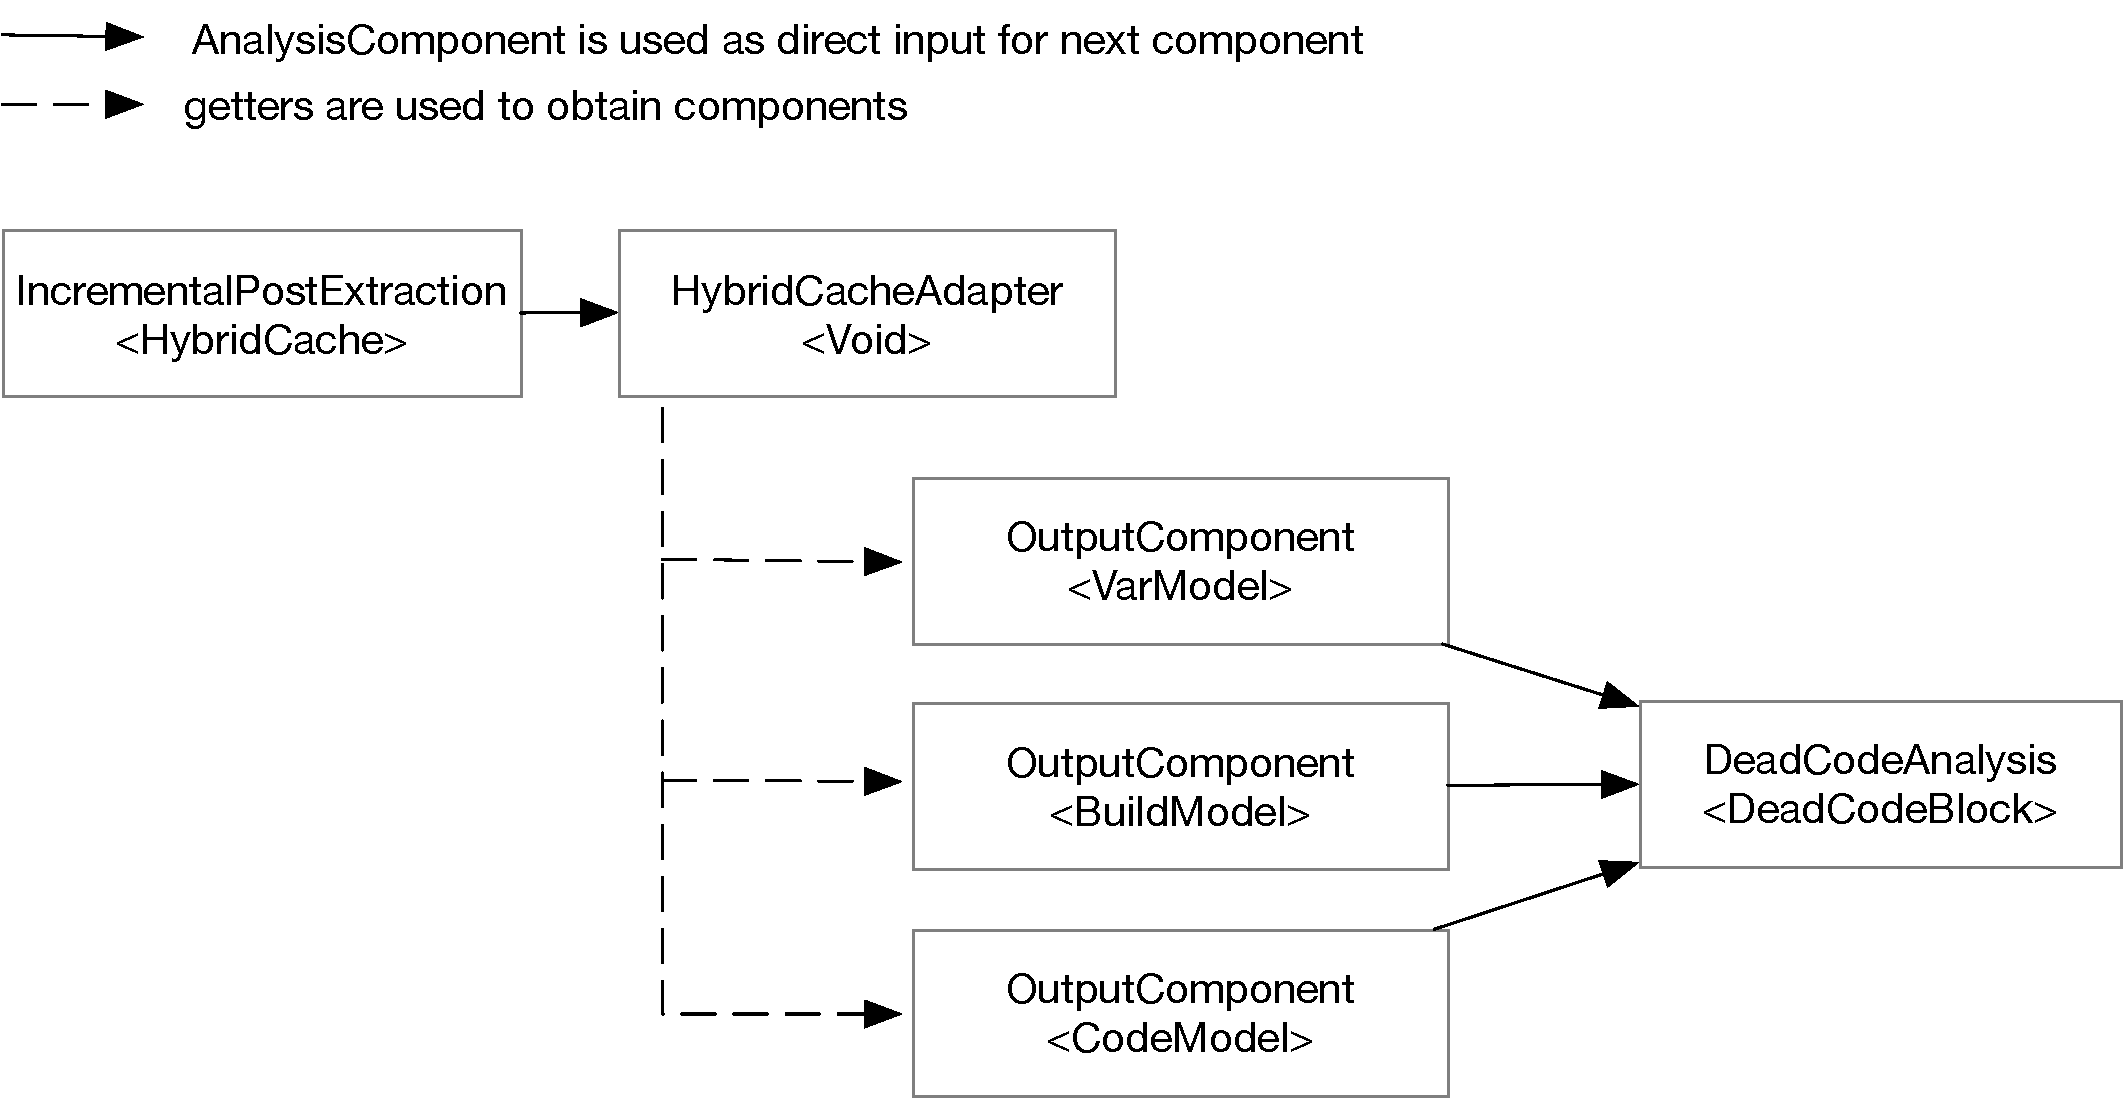
\includegraphics[width=1\textwidth]{img/HybridCacheAdapter.pdf}
  \end{minipage}
\end{figure}

Adapting the input for the analysis is not the only purpose of the \texttt{Hybrid\-Cache\-Adapter} as it also defines which parts of the code model are passed on to the \texttt{Analysis\-Component}. Some  \texttt{Analysis\-Component}s like the \texttt{FeatureEffectAnalysis} \cite{feature-effect-analysis}\cite{Nadi15wheredo} might always need the complete code model and are therefore able to profit from faster extraction times through the incremental infrastructure. In fact any existing non-incremental analysis for KernelHaven is able to process complete models as this is what the KernelHaven infrastructure provides by default. It is therefore worth noting that the easiest way to benefit from the incremental infrastructure is to pass the entire build, code and variabilitymodel to the analysis through the \texttt{Hybrid\-Cache\-Adapter}. While this does not yield any performance benefits for the analysis defined through the code within the analysis plugin itself, it potentially shortens the required time for model extraction.

However the \texttt{Dead\-Code\-Analysis} may only need to access the part of the model that was modified as processing unchanged parts of the model does not always induce new results. Therefore the \texttt{Hybrid\-Cache\-Adapter} can either be used to return a complete code model or just the changed parts. The implementation of an incremental version of the \texttt{Dead\-Code\-Analysis} itself is explained in the next section.

As the \texttt{Hybrid\-Cache\-Adapter} is meant for quick adaptation of existing analyses, it only provides generic functionality for filtering the code model by allowing to only provide the changed parts of the model. If filters are specifically designed to work for one analysis, they should be implemented within that analysis itself utilizing the full capabilities of \texttt{Hybrid\-Cache} instead of relying on an adapter. This is why in contrast to \texttt{Incremental\-Preparation} where custom implementations for \texttt{InputFilter}s are allowed for filtering files within the codebase, the \texttt{Hybrid\-Cache} does not provide such an interface for filtering the code model.

\subsubsection{Incremental dead code analysis} \label{incremental-dead-code-analysis}

The \texttt{Dead\-Code\-Finder} is an \texttt{Analysis\-Component} implemented in the \texttt{UndeadAnalyzer}-plugin of KernelHaven. It uses the code-, build- and variabilitymodel to compute results. The code model is represented by a collection of \texttt{Source\-File}-objects each representing the model of a single sourcefile from the codebase.

The analysis iterates over all \texttt{Source\-File}-objects and separately checks them for dead code blocks. The constraints defined through the build- and variabilitymodel are included for the identification of such code blocks. Because every model represented by a \texttt{Source\-File} is considered separately, changes in other parts of the code model do not impact the result of an unchanged parts. Therefore unchanged parts of the model do not need to be analyzed again if only the code model changed. It is sufficient to only analyze the parts of the code model that did change.

If however the variability or the build model did change, the restrictions that were used to analyze the each part of the code model have changed aswell. As a result, the entire code model has to be processed again within the analysis.

Therefore for implementing an incremental version of the \texttt{Dead\-Code\-Analysis} we have to consider the following two possibilities:

\begin{enumerate}
 \item variabilit and build model did not change
 \begin{itemize}
 	\item only provide newly extracted parts of the code model to \texttt{Dead\-Code\-Finder}
 \end{itemize}
  \item variability and/or build model did change
 \begin{itemize}
 	\item provide complete code model to \texttt{Dead\-Code\-Finder} (including parts of the model that were extracted in previous executions of the incremental analysis)
 \end{itemize}
\end{enumerate}

The current variability and build model are always provided to the \texttt{Dead\-Code\-Finder} as they are required to process each \texttt{Source\-File}-object. The following code shows the main part of the incremental implementation for the dead code analysis\footnote{for the complete implementation refer to \url{https://github.com/KernelHaven/IncrementalDeadCodeAnalysis}}:

\begin{lstlisting}[language=java]
// Determine whether only a part of the code model must be analyzed
if (!updatedBuildModel && !updatedVariabilityModel) {
    cmProcessing = code modelProcessing.PARTIAL;
} else {
    cmProcessing = CodeModelProcessing.COMPLETE;
}

// Create the adapter
HybridCacheAdapter hca = new HybridCacheAdapter(config,
    new IncrementalPostExtraction(config, 
        getCmComponent(), 
        getBmComponent(), 
        getVmComponent()
    ),
    cmProcessing);

// Create the AnalysisComponent performing the dead code analysis
DeadCodeFinder dcf = new DeadCodeFinder(config, 
    hca.getVmComponent(), 
    hca.getBmComponent(),
    hca.getCmComponent());

return dcf;
\end{lstlisting}

\newpage
\section{Evaluation}\label{evaluation}

The evaluation of the incremental infrastructure will be performed to measure the performance gain as well as to confirm the constistency of the results with those of a non-incremental analysis. The incremental infrastructure with the dead code analysis will be compared against the non-incremental dead code analysis implemented for KernelHaven. Both systems will be using the same configuration for execution with the exception being the additional parameters required for incremental analyses and of course the analysis-class itself. The exact configurations used are described in the Appendix.

After computing some first preliminary results using both the incremental infrastructure and a non-incremental analysis in KernelHaven, it became clear that the evaluation could not be performed for a large set of commits in a timely manner without further changes. This is because the non-incremental analysis always has to perform SAT-solving for all of the conditions imposed by the models for each commit. Both the machine used for development with two CPU cores and 16GB RAM as well as the most powerful machine accessible for us with 40 CPU cores and 300GB of RAM were only able to perform about three iterations of the analysis per day. However, the existing dead code analysis was not multithreaded.  s. In doing so, we were able to achieve appoximately 35 analyses per day on our reference system. Those changes enabled the timely availabily of reference results for the incremental analysis to compare against. In order to keep the results compareable, the incremental version of the analayis was also adjusted to support multithreaded operation. 

The data used for evaluation consists of 307 commits to the main branch of the Linux Kernel source tree \cite{linux}. Each commit was transformed into a git-diff file that then was directly used as input for the incremental analysis. The non-incremental reference results were also computed based on the diff-files. However the changes described through each git-diff file were applied to the codebase before the execution of KernelHaven itself as the non-incremental dead code analysis expects a codebase that it can work with directly. Therfore the incremental executions contain an elemenent within their executions that was externalized for non-incremental executions. The table below shows the exact range of commits used and how they were represented for the evaluation.

\begin{tabular}{l | l | l}
	Commit-Hash & Description & File \\ \hline
	4fbd8d194f06c8a3fd2af1ce560ddb31f7ec8323 & Linux 4.15-rc1 & 00001-git.diff \\
	... & ... & ... \\
	d8a5b80568a9cb66810e75b182018e9edb68e8ff & Linux 4.15  & 00307-git.diff \\
\end{tabular}

To automate the generation of results, a collection of bash-scripts and is available within a the github-project Incremental\-Analyses\-Evaluation\footnote{\url{https://github.com/moritzfl/IncrementalAnalysesEvaluation}}. Incremental\-Analyses\-Evaluation also includes the git-diff files and  configuration files used for evaluation along with the results computed by KernelHaven within the release section of the repository. The reference system used for execution was a virtual linux machine hosted on VMware ESXi\footnote{\url{https://www.vmware.com/products/esxi-and-esx.html}} with 24 configured CPU-cores and 64GB RAM while the host system itself had access to 12 phyisical and 24 logical CPU cores clocked at 2.20 GHz each. The CPU model used was an Intel Xeon E5-2650. The JVM was started using the options \texttt{-Xms10G} and \texttt{-Xmx50G}.

\subsection{Early Evaluation Results} \label{early-evaluation-results}

For obtaining evaluation results, we used the results of a non-incremental dead code analysis as reference.  The reference (Ref) was compared against two incremental analyses that were configured according to the \texttt{variability-change-only} (VarChange) and a \texttt{change-only} options (Change) described by REQ \ref{req:mandatory-filters}.
When running the evaluation, some issues were identified that needed to be fixed. Therefore the results of the incremental executions (Change, VarChange) were not entirely consistent with Ref. However they were close enough to assume that resolving those issues would produce consistent results. Given that the results were inconsistent, no evaluation of the performance was performed at this point.

The first issue that was noticed was that the execution of the bash-script for Ref stopped unexpectedly. The interruption occured when applying the changes described by the file \texttt{00129-git.diff} to the codebase. This is because this file is empty as the commit it represents was a merge-commit to the main branch of the Linux Kernel that did not actually change anything. Therefore the commit was skipped for all subsequent evaluation executions.

Looking at the isolated results of Ref, it became clear that Ref had issues analyzing some states of the codebase. A total of 71 Ref executions resulted in no dead code blocks. However, all preceding and subsequent analysis results contained dead code blocks. When investigating the log-files we found that the issue was most likely due to the \texttt{KConfigReaderExtractor} not being able to extract the model from the codebase. Upon further investigation and using the original KConfigReader-tool, the assumed cause was confirmed. In the KConfig language the keyword \texttt{choice} is used to describe a set of alternative configuration options. While the KConfig language allows a \texttt{choice} to be empty (eventhough an empty choice does not make sense), KConfigReader expects configuration options to be present when the keyword \texttt{choice} is used. 

However the KConfigReader bug revealed a related bug for the incremental executions as those did still find dead code blocks. This is because when the extraction of variability and build model failed, the incremental infrastructure provided the previous models to the analysis. It was implemented in a way that it only replaced old models with new one - and if no new models were extracted the old ones were simply kept. This has now been fixed as a failed execution of the build model or variabilitymodel now results in the deletion of the model from the \texttt{Hybrid\-Cache}\footnote{rollback is still possible}.

Additionally, a bug within the \texttt{VariabilityChangeFilter} was found that resulted in files not being marked as \texttt{VariabilityChange.CHANGE} in cases where ComAn could not extract variability information. While this is only relevant for a small number of cases, this behaviour represents an important fallback mechansism. A false negative might result in files not being considered for extraction while they did in fact change variability. Preventively marking them as \texttt{VariabilityChange.CHANGE} results in those files being processed by the extractors and ensures that the extracted model they represent is consistent with the codebase. While marking files as \texttt{VariabilityChange.CHANGE} potentially increases the computational effort in case of a false positive, it thereby also ensures the availability of correct models for the analysis. Correct models are of paramount importance for achieving consistent results. Therefore it is better to risk a false positive than a false negative. In this instance however the bug had no actual impact on the consistency of results. This is because the only entries within the git-diff files that were identified as problematic for the ComAn-tool were either affecting binary files or additions of empty files and no files containing actual changes to variability.

In the concept for incremental analyses, we handled the extraction of code, build and variability model als separate concerns. While this makes sense in theory and may even be applicable for future extractor plugins for KernelHaven, the \texttt{KbuildMinerExtractor} uses the variability model to differenciate between boolean and tristate variables. Therefore the extraction of the build model is dependent on the variability model. When handling build and variability model separately, inconsistencies may appear when a boolean variable is converted into a tristate variable or vice versa. This issue has been resolved by always performing an extraction of the build model when the variability model changes. There is however room for optimization as the extraction of the build model is only necessary in the described corner case when all of the following conditions are met:

\begin{itemize}
	\item the type of a variable is changed
	\item files related to the variability model were included after filtering
	\item no files related to the build model were included after filtering 
\end{itemize}   

In fact the inconsistency was only visible for the analysis result of one single commit within the 306 analyzed commits\footnote{as explained in earlier in this section, \texttt{00129-git.diff} was skipped}. However there were also expected deviations within the results of the variabilty-only-filter execution compared to the reference. Using the \texttt{Variability\-Change\-Filter}, the code model for a single codefile only gets rebuilt when variability-information within that file is modified. When a change is made within a codefile that does not change variability-information, it might still change the position of dead code blocks. A trivial example would be an inserted comment line right before an \texttt{\#ifdef}-block. This moves the block down by one line. However the code model does not get extracted again. The code model still contains the information that \texttt{\#ifdef}-blocks exist within the same codefile but only has access to the previous linenumber. As a result, when an analysis is performed on the entire code model after an update to the build- or variabilitymodel, the linenumbers do not match the result of the reference. A solution for this would be to modify the code model within the \texttt{Hybrid\-Cache} using information from the git-diff file. The git-diff file can be used to determine at which positions within the files modifications were made. Therefore if the variability information did not change, we can assume that the addition of a few lines of code increases the number of the start line and end line of all subsequent codeblocks by the number of lines that was added. If lines are added within a codeblock it only changes the linenumber for its end position but both the linenumbers of start and end position for all subsequent code blocks. This has however not been implemented yet.

Another deviation from the reference result stems from the fact that only variabilty-changes are considered to be relevant. In the reference execution, a dead code analysis was performed covering every single sourcefile in the codebase. This is not the case for the VarChange execution as it only covers the files where variability-information was modified.

The following entry was present in the reference result for \texttt{00001-git.diff} but not for the incremental result using the \texttt{VariabilityChangeFilter}:

\begin{lstlisting}
drivers/net/arcnet/com90xx.c;(CONFIG_ARCNET_COM90xx || CONFIG_ARCNET_COM90xx_MODULE) && (CONFIG_ARCNET || CONFIG_ARCNET_MODULE);606;610;0
\end{lstlisting}

Looking at \texttt{drivers/net/arcnet/com90xx.c} we can see that the dead code block actually got inserted on purpose and does not represent a modification to variability:

\begin{lstlisting}
#if 0
    /* don't do this until we verify that it doesn't hurt older cards! */
    arcnet_outb(arcnet_inb(ioaddr, COM9026_REG_RW_CONFIG) | ENABLE16flag, ioaddr, COM9026_REG_RW_CONFIG);
#endif
\end{lstlisting}

The reference results therefore contained more dead code blocks as they also included those from files where the variability was not changed. However when ignoring additional entries for non-variablity-related dead code blocks within the reference results, the variability-change-only results matched the reference results. Relevant entries that are related to variability can be identified because their presence condition has to contain the \texttt{CONFIG\_} prefix. In the result the presence condition is denoted as the element behind the last semicolon. In our example the presence condition is \texttt{0}. It does not contain \texttt{CONFIG\_} and therefore is not related to variability.

Considering the results, the variability-change-only option is suitable when dead code blocks related to variabilty are the major concern. If however all dead-code-blocks should be found, one should be able to use the \texttt{ChangeFilter} for the code model instead. That way, all changes within the code model get analyzed while changes to build- and variabilitymodel are still processed using the \texttt{VariabilityChangeFilter}. This configuration seems practical, because the extraction and analysis of single codefiles does only require a small computational effort. However updates to the build- or variabilitymodel would result in costly computations as they require a full analysis covering the entire code model.

\subsection{Final Evaluation Results}

This section covers the evaluation results obtained after performing the modifications resulting of the findings described within Section \ref{early-evaluation-results}. We will first provide an overview over the results and performance of the incremental configurations (Change, VarChange) compared to Ref before taking a deeper look at the performance of individual executions in Section \ref{individual-performance}. Finally, we will also compare Ref against a non-incremental analysis execution performed within the incremental infrastructure in Section \ref{evaluation-filteroff}. 

After implementing the alterations described in Section \ref{early-evaluation-results}, we were able to achieve results that were consistent with the reference. This means that for Change, the following statements can be made:

\begin{itemize}
   \item Each result contained at least all dead code blocks that were present in the reference result for the same diff-file but not in the reference result for the previous one
   \item No result contained dead code blocks that were not present in the reference result for the same diff-file
\end{itemize}

When ignoring line numbers and all dead code blocks that did not include a KConfig variable in their presence condition, the same is true for the VarChange configuration. 

Given that the results now are consistent with the reference, we continued to evaluate the performance gain. \autoref{tab:performance} shows the average performance per execution phase Change, the VarChange and the Ref. The performance data was generated by analyzing the timestamps of each log file. The timestamps within log files of KernelHaven have a resolution of one second. While it can be argued that this precision is relatively low for performance measurements, it suffices for this comparison because the durations measured for the reference lie within minutes or hours.

\begin {table}[h]
\begin{center}
\caption {Average Performance by Phase (Change, VarChange, Ref)} \label{tab:performance} 
\begin{tabular}{|l | l | l | l|}
\hline
                               & Change                 & VarChange          & Ref  \\ \hline
	Preparation                & 0.072 s                & 11.72 s            & 0.00 s \\
	\underline{E}xtraction     & 26.22 s                & 11.70 s            & 608.80 s \\
	\underline{A}nalysis       & 407.94 s               & 157.25 s           & 1792.80 s \\
	\underline{O}verlap        & 0.00 s                 & 0.00 s             & 501.45 s \\
	E + A - O                  & 434.16 s               & 168.95 s           & 1900.15 s \\
	Post-Extraction             & 1.91 s                 & 0.50s              & 0.00 s \\ \hline
	Total                      & 7 min 16 s             & 3 min 2 s          & 32 min 47 s \\ \hline
\end{tabular}
\end{center}
\end{table}

The Preparation-Phase was identified by log entries that directly marked the start and end of the phase. For the Extraction-Phase, we defined the start of the phase through the line where an extractor thread first produced an output and the end through the last line within the log where an extractor announced that all its threads are done. The Analysis phase was identified by the first occurence of a line where the class \texttt{OrderPreservingParallelizer} produced output. This class is responsible for the multithreaded SAT-solving that the dead code analysis requires and indicates that the analysis started processing the models. The end of the Analysis-Phase was identified through the log line where the KernelHaven infrastructure announced that the analysis has finished. The time between Extraction-Phase and the Analysis-Phase is interpreted as Post-Extraction-Phase. According to our interpretation of Analysis-Phase and Extraction-Phase for the measurements, the Post-Extraction-Phase includes the time that the \texttt{Hybrid\-Cache\-Adapter} needs to make the models available to the dead code analysis. The total execution time was measured through the difference in time between the first and the last log entry. While they are included in the total duration, we did not list tasks outside of the four phases outlined in Section \ref{4-phases} separatly (e.g. loading of plugins before the Preparation-Phase starts).

In non-incremental executions, analyses can directly use the output of the extractors as soon as they generate a result. While build and variability model extractors can only provide complete models, the code model extractor can provide the code model in parts. As mentioned in Section \ref{kernelhaven}, each part of the code model that represents a single code file can be extracted separately. This allows the code extractors to make the code model available to the analysis piece by piece.
After the results of build and variability extractors become available, the non-incremental dead code analysis starts looking for dead code blocks. It achieves this by using the parts of the code model that  have already been extracted. Meanwhile the code extractor continues to extract the rest of the code model. Because the analysis may already start before all extractors have terminated, this creates an overlap between Analysis and Extraction-Phase. The incremental infrastructure on the other hand waits for the extractors to first provide all models and then merges newly extracted models with the previous models before making them available to the analysis. Therefore the non-incremental dead code analysis has to wait with its computations until all models are available through the HybridCache and thus does not have any overlap between phases. In order to offer a more comparable value between the different configurations, the table also shows the duration of both phases together with the overlap removed (E + A - O). 


The results show that the incremental executions are significantly faster on average than the reference counterpart. The change-only executions only took about 22\% of the time compared to the reference executions while variability-change executions achieved even faster execution times requiring only 9\% of the reference execution time.

\subsubsection{Individual Performance per Execution}\label{individual-performance}

After evaluating the overall performance using the average values, this section focuses on differences between individual execution times. \autoref{fig:change} shows the duration of the executions of Change and Ref for all states of the codebase as described by the respective git-diff files. We can see that Change often achieved results close to the horizontal axis thereby indicating fast execution times. When only code files were changed, the \texttt{ChangeFilter} ensured that the dead code analysis only had to identify dead code blocks within the modified code files. In fact 78\% of all executions were such partial analyses that took only about 7s on average. This percentage matches the findings of Kr\"oher and Schmid \cite{ComAn} who found that 78.29\% of commits change code files exclusively. However the other 22\% of executions required a full dead code analysis covering the entire code model. Such an execution is far more costly and took 2001 s on average. 

The relatively low execution times between commit nr 46 and 116 can be explained through the \texttt{choice} bug identified in Section \ref{early-evaluation-results}. For those commits, no actual dead code analysis could be performed because the models were incomplete. Nevertheless, we chose to include the results for our evaluation as they do still demonstrate the differences between incremental and non-incremental executions. While Ref always tried to extract all models, Change only tried to extract the changed parts thereby being able to terminate faster. 


\begin{figure}[h] 
  \centering
  \begin{minipage}[b]{1\textwidth} 
    \caption[Change Performance]{Change compared to Ref Performance}\label{fig:change}
    \centering
    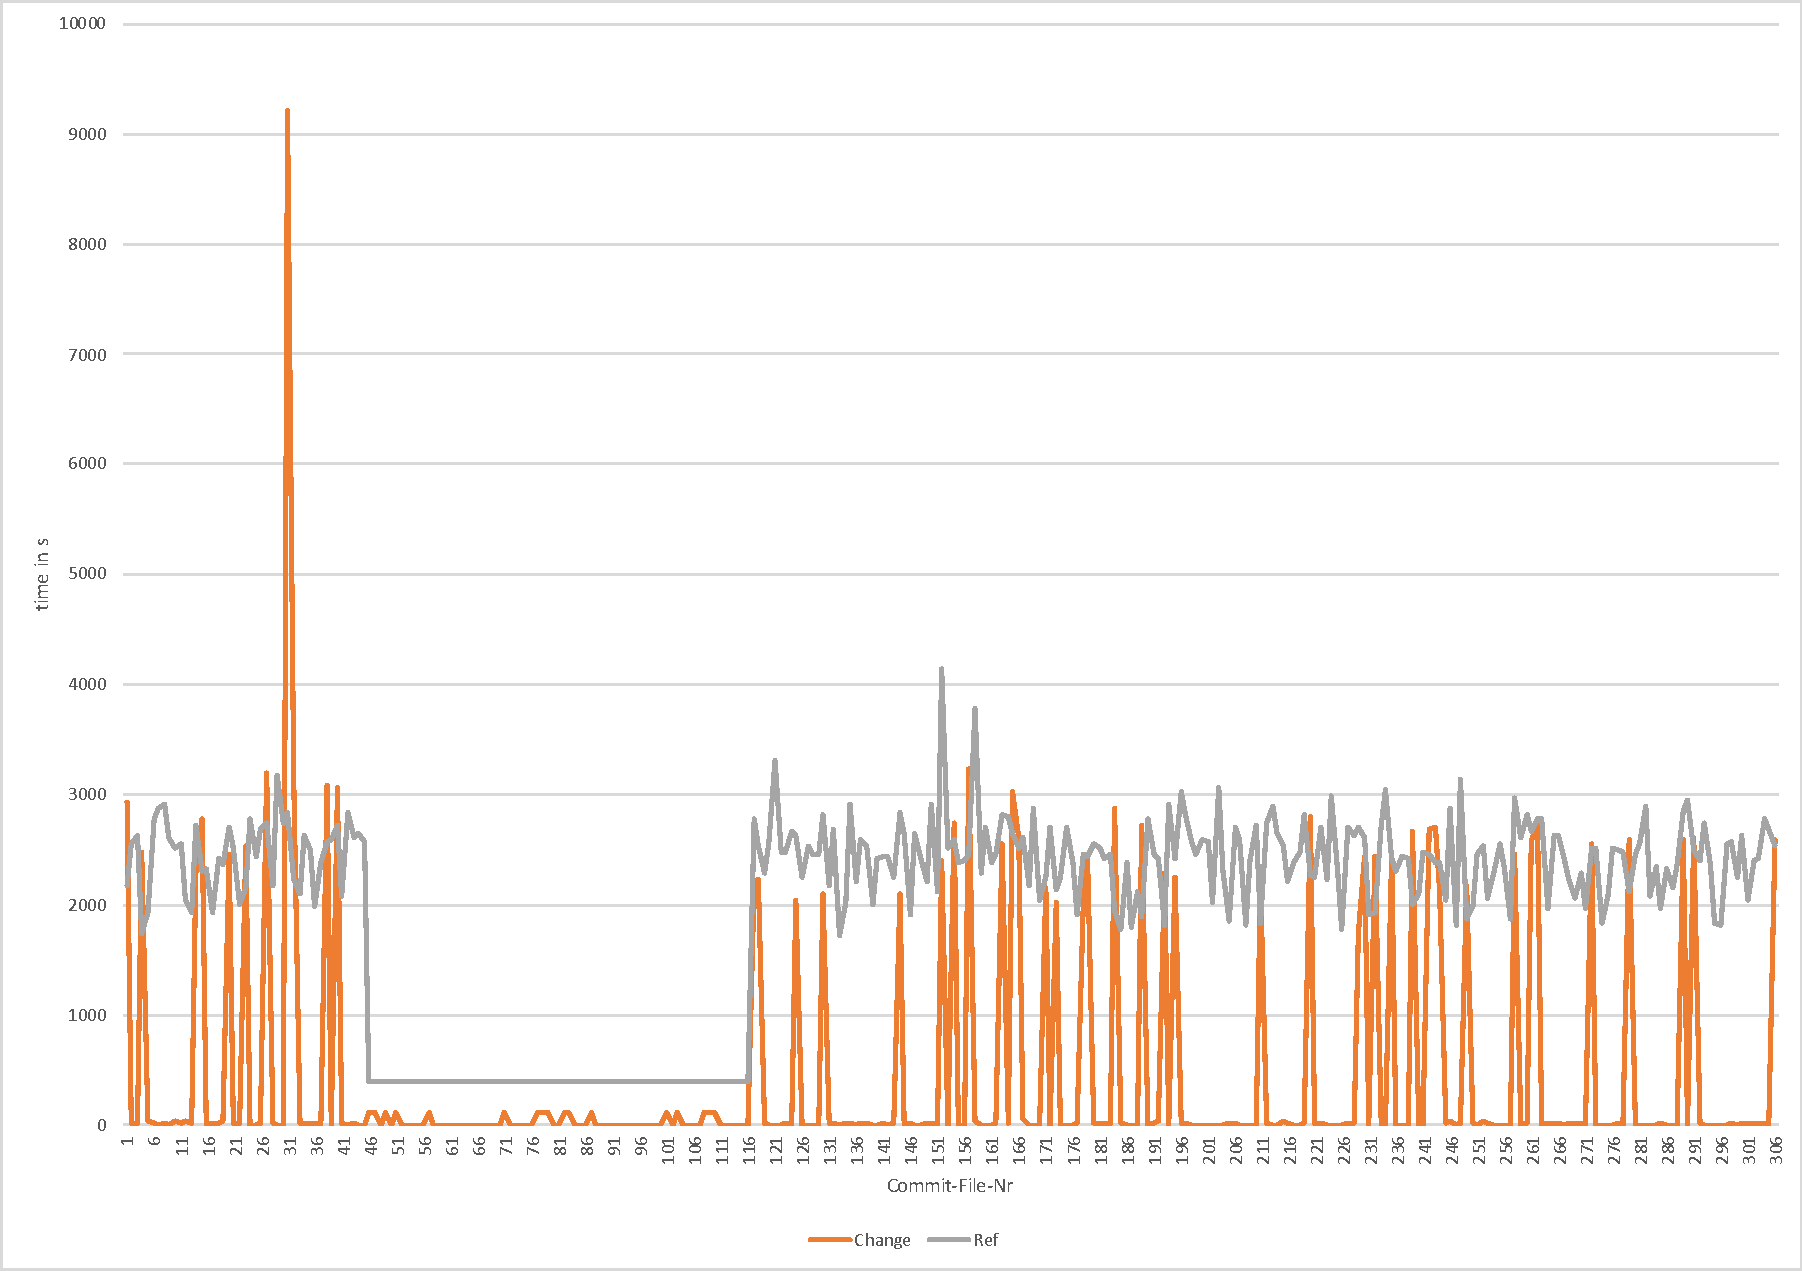
\includegraphics[height=1\textwidth, angle=90]{img/change-vs-ref.pdf}
  \end{minipage}
\end{figure}


For all except one analysis execution, Change achieved better or compareable performance to Ref. However the one outlier apparently required much longer than all other executions. The outlier represents the execution based on \texttt{00031-git.diff}. In theory no Change execution should be significantly slower than the first execution as the first execution has to process the initial commit to the codebase and perform a full analysis based on the complete code, build and variability model. While other subsequent executions might still require a full analysis, they do not have to perform a full extraction of the entire code model as only the modified code files need to be processed by the extractor. 
Looking at the specific log file, we also found that the duration of the Extraction-Phase was above average but still reasonably quick at 75s. The only execution phase with a significantly long duration was the Analysis-Phase measuring in at about 2h 31min ($\approx 9000s$). As the incremental dead code analysis uses the same AnalysisComponent from the UnDeadAnalyzer plugin as the reference analysis, the component should operate at the same speed once the models are provided. Therefore we were unable to find reasons for the outlier within our implementation. We repeated the analysis execution for the changes described by \texttt{00031-git.diff} in order to be able to consult date from more than one execution. The additional five executions performed for \texttt{00031-git.diff} had an average execution time of 2794 s which falls within the normal range as depicted in the plot. This hints at external reasons for the prolonged execution time - however we were unable to identify the exact reason for the outcome of the initial measurement.

The curve for Ref is rather unstable between analysis executions. We assume randomized procedures within the SAT-Solver to be the cause for this. Because the Analysis-Phase in which SAT-solving is performed is the most time consuming phase, variations within this phase make it difficult to draw further conclusions. After all the incremental executions are also affected by the randomization effects of the SAT-Solver. Therefore a full incremental analysis is sometimes faster and sometimes slower than a reference analysis. Compared to Change, Ref was faster for 29 out of the 66 iterations where Change performed a full analysis. This seems to indicate that the execution times for full analyses within Change and analyses within Ref do not have a noteworthy difference in overall performance.

\begin{figure}[h] 
  \centering
  \begin{minipage}[b]{1\textwidth} 
    \caption[VarChange Performance]{VarChange compared to Ref Performance}\label{fig:var-change}
    \centering
    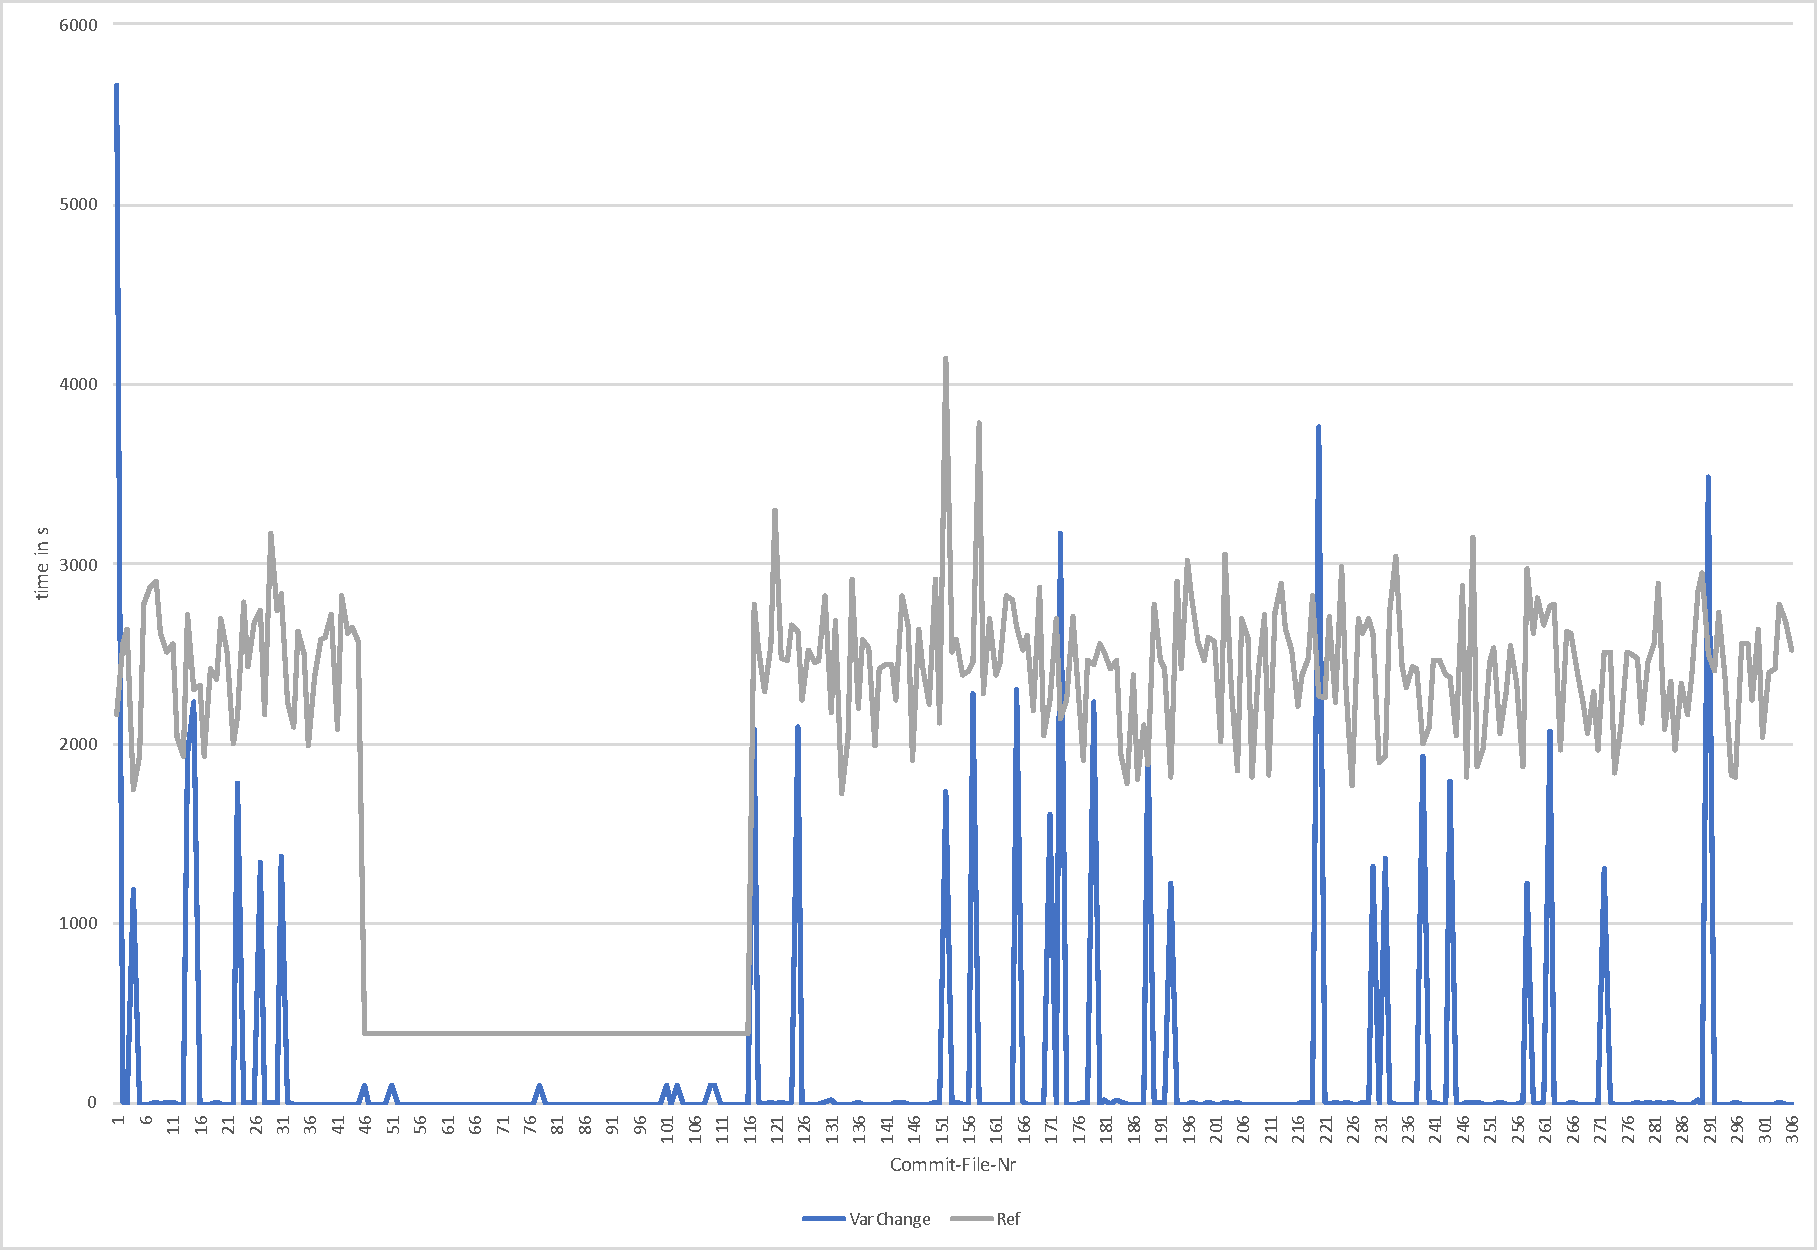
\includegraphics[height=1\textwidth, angle=90]{img/var-change-vs-ref.pdf}
  \end{minipage}
\end{figure}

\autoref{fig:var-change} shows the execution times of VarChange compared to Ref. Similar to Change, VarChange also produced either much lower or comparable execution times compared to Ref. Only the first execution of VarChange took noticeably longer than Ref. In contrast to our outlier in the Change iteration however, this has a rather simple explanation. As mentioned in \autoref{preparation-phase} the \texttt{Variability\-Diff\-Analyzer} takes a significant amount of time (about an hour) to analyze the first git-diff file. After the first execution, all subsequent analysis executions only need to process a relatively small git-diff file and therefore do not require as much time in the Preparation-Phase.  Overall VarChange was able to perform partial analyses for 89\% of all executions with an average duration of about 2 s per partial execution. For the other 11\% where full analyses were required, VarChange took about 1674s on average. In contrast to Change, the results for VarChange seem to indicate that VarChange is also faster than Ref when performing full analyses. In total Ref was faster for only 5 out of 33 full analysis executions that were performed for VarChange. A possible explanation for this would be that a smaller subset of codefiles is checked for dead code. If the \texttt{VariabilityChangeFilter} does not find any variability information within a code file, the code file is also not considered fo model extraction. Therefore the resulting code model is smaller and thereby offers less targets for the dead code analysis to work on. Therefore VarChange can potentially finish faster even when a full analysis based on the entire available code model is required.

\begin{figure}[h] 
  \centering
  \begin{minipage}[b]{1\textwidth} 
    \caption[VarChange compared to Change Performance]{VarChange compared to Change Performance}\label{fig:var-change-vs-change}
    \centering
    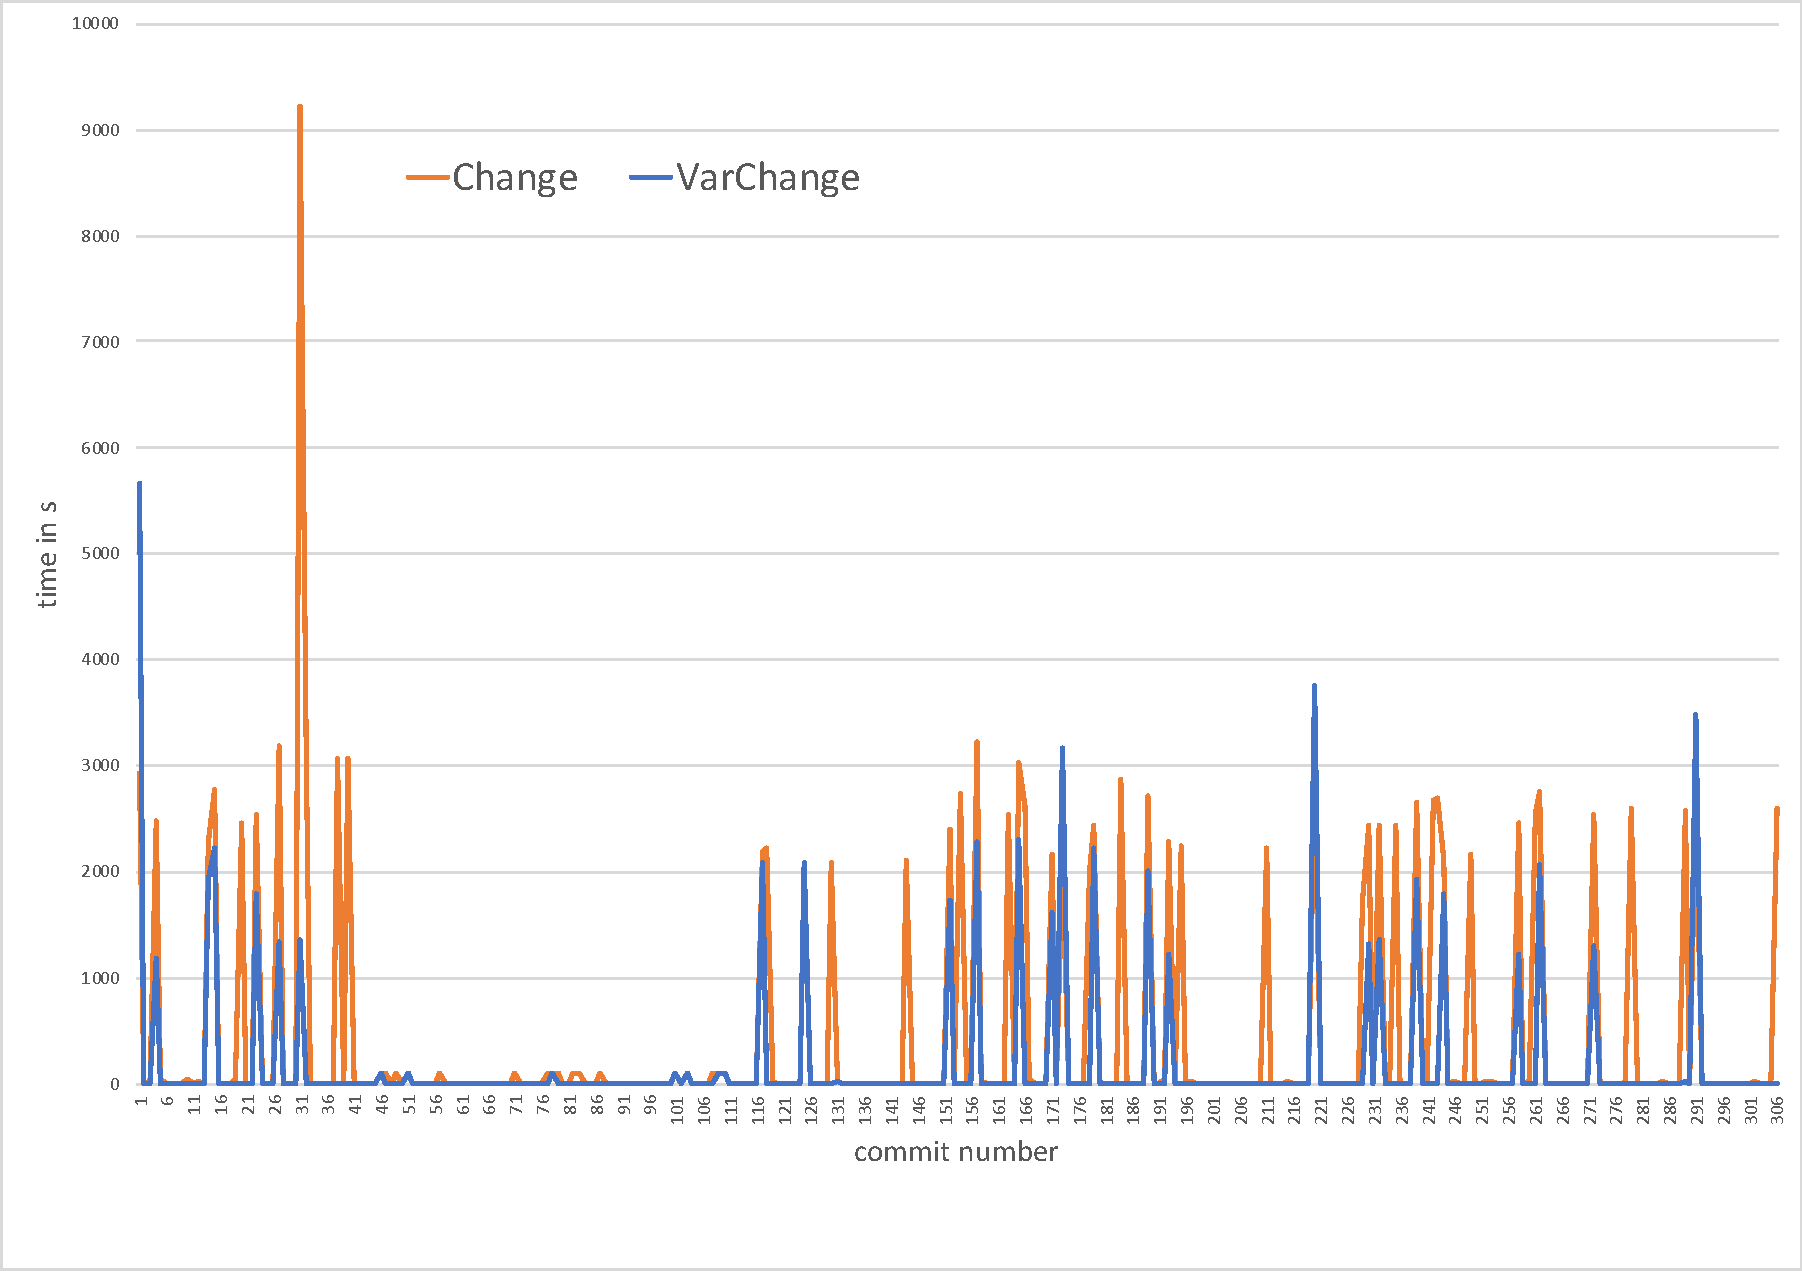
\includegraphics[height=1\textwidth, angle=90]{img/var-change-vs-change.pdf}
  \end{minipage}
\end{figure}


Finally \autoref{fig:var-change-vs-change} shows the results of VarChange and Change together. It is worth highlighting at this point that with 11\% of executions requiring a full analysis, VarChange was able to reduce the number of spikes compared to the 22\% for Change. Therefore the plot often shows spikes for Change while no spikes for VarChange appear for the same git-diff file.
The plot also indicates that VarChange executions might be faster on avererage when considering only those data points where a full analysis was required for VarChange. Investigating the perfomance results more closely, we found that VarChange was faster for 23 out of the 33 executions where it required a full analysis when compared to Change. This seems to support the hypothesis that VarChange is faster in those cases but the difference is not big enough to provide a definitive answer considering the small size of our dataset.
 
 \clearpage
 \newpage
\subsubsection{Results of the Incremental Infrastructure without Filtering}\label{evaluation-filteroff}

After evaluating Change and VarChange, we compared Ref with a configuration representing the \texttt{off} option described through REQ \ref{req:mandatory-filters} (FilterOff). An execution with this configuration always performs a full analysis and does not reduce the number of files processed. Therefore all analysis results produced by FilterOff do exactly match the results of Ref without any deviation. Because for FilterOff the extractors have to process the same part of the codebase and the analyses have to process the same models as Ref, this comparison allows us to draw conclusions concerning the performance cost of mandatory tasks within the incremental infrastructure.

\begin {table}[h]
\begin{center}
\caption {Average Performance by Phase (FilterOff, Ref)} \label{tab:performance-filteroff} 
\begin{tabular}{|l | l | l|}
\hline
                               & FilterOff                   & Ref  \\ \hline
	Preparation                & 1.42 s                      & 0.00 s \\
	\underline{E}xtraction     & 396.59 s                    & 608.80 s \\
	\underline{A}nalysis       & 1800.78 s                   & 1792.80 s \\
	\underline{O}verlap        & 0.00 s                      & 501.45 s \\
	E + A - O                  & 2197,37 s                   & 1900.15 s \\
	Post-Extraction            & 3.06s                       & 0.00 s \\ \hline
	Total                      & 36min 42s                   & 32 min 47 s \\ \hline
\end{tabular}
\end{center}
\end{table}

\autoref{tab:performance-filteroff} shows the average performance of FilterOff compared to Ref. According to the results, FilterOff took about 112\% of the time that Ref took. We can also see that neither Preparation-Phase nor Post-Extraction-Phase introduced a significant performance cost. The computational effort for the Analysis-Phase does not seem to differ between FilterOff and Ref as the measured results only showed a neglectable difference of about 1\%. However the Extraction-Phase was much faster for FilterOff taking only about 65\% of the time that the Extraction-Phase took within Ref. Therefore the difference in performance seems to stem entirely from the overlap between Extraction-Phase and Analysis-Phase within Ref. The overlap allows the non-incremental dead code analysis to start processing the results earlier thereby offering an advantage for Ref in this instance. 

While this seems like a potential benefit for non-incremental analyses when compared to incremental analyses, we would argue that it is not relevant for practical implementations. As the numbers shown in \autoref{tab:performance} indicate, we were able to achieve significant performance gains within the Extraction-Phase for both Change and VarChange executions where the average Extraction-Phase finished within seconds on average. Those gains are mostly due to being able to perform partial extractions of the code model and merge the result back with the result of previous extractions. In fact, the extraction of the code model takes less time than an extraction of build and variability model for almost every VarChange or Change execution. Therefore it could be argued that the measured difference in performance between FilterOff and Ref loses most of its relevance. 

Interestingly, this assumption however does not seem to be supported by the average performance for full extractions of Change (2001 s) compared to Ref (1967 s). However the average values for full extractions were assessed including the executions where the \texttt{KConfig\-Reader\-Extractor} failed to extract the model. Because Ref always has to perform a full analyses, all of those iterations were considered full analyses - after all, Ref \emph{tried} to work with all three models. Change on the other hand only was considered to be performing a full analysis when either build or variability model had to be extracted again. The relatively low duration of those iterations contributes to a lower average execution time. Because Change only included a total of 66 full analyses, the impact of one of the executions lying within the range affected by the \texttt{KConfig\-Reader\-Extractor} bug is rather large. On the other hand, all of those executions are included for the FilterOff configuration. Therefore the comparison of the average execution time for full analyses between FilterOff and Ref does not necessarily contradict our assumption. 

\begin{figure}[h] 
  \centering
  \begin{minipage}[b]{1\textwidth} 
    \caption[FilterOff compared to Ref Performance]{FilterOff compared to Ref Performance}\label{fig:filteroff-vs-ref}
    \centering
    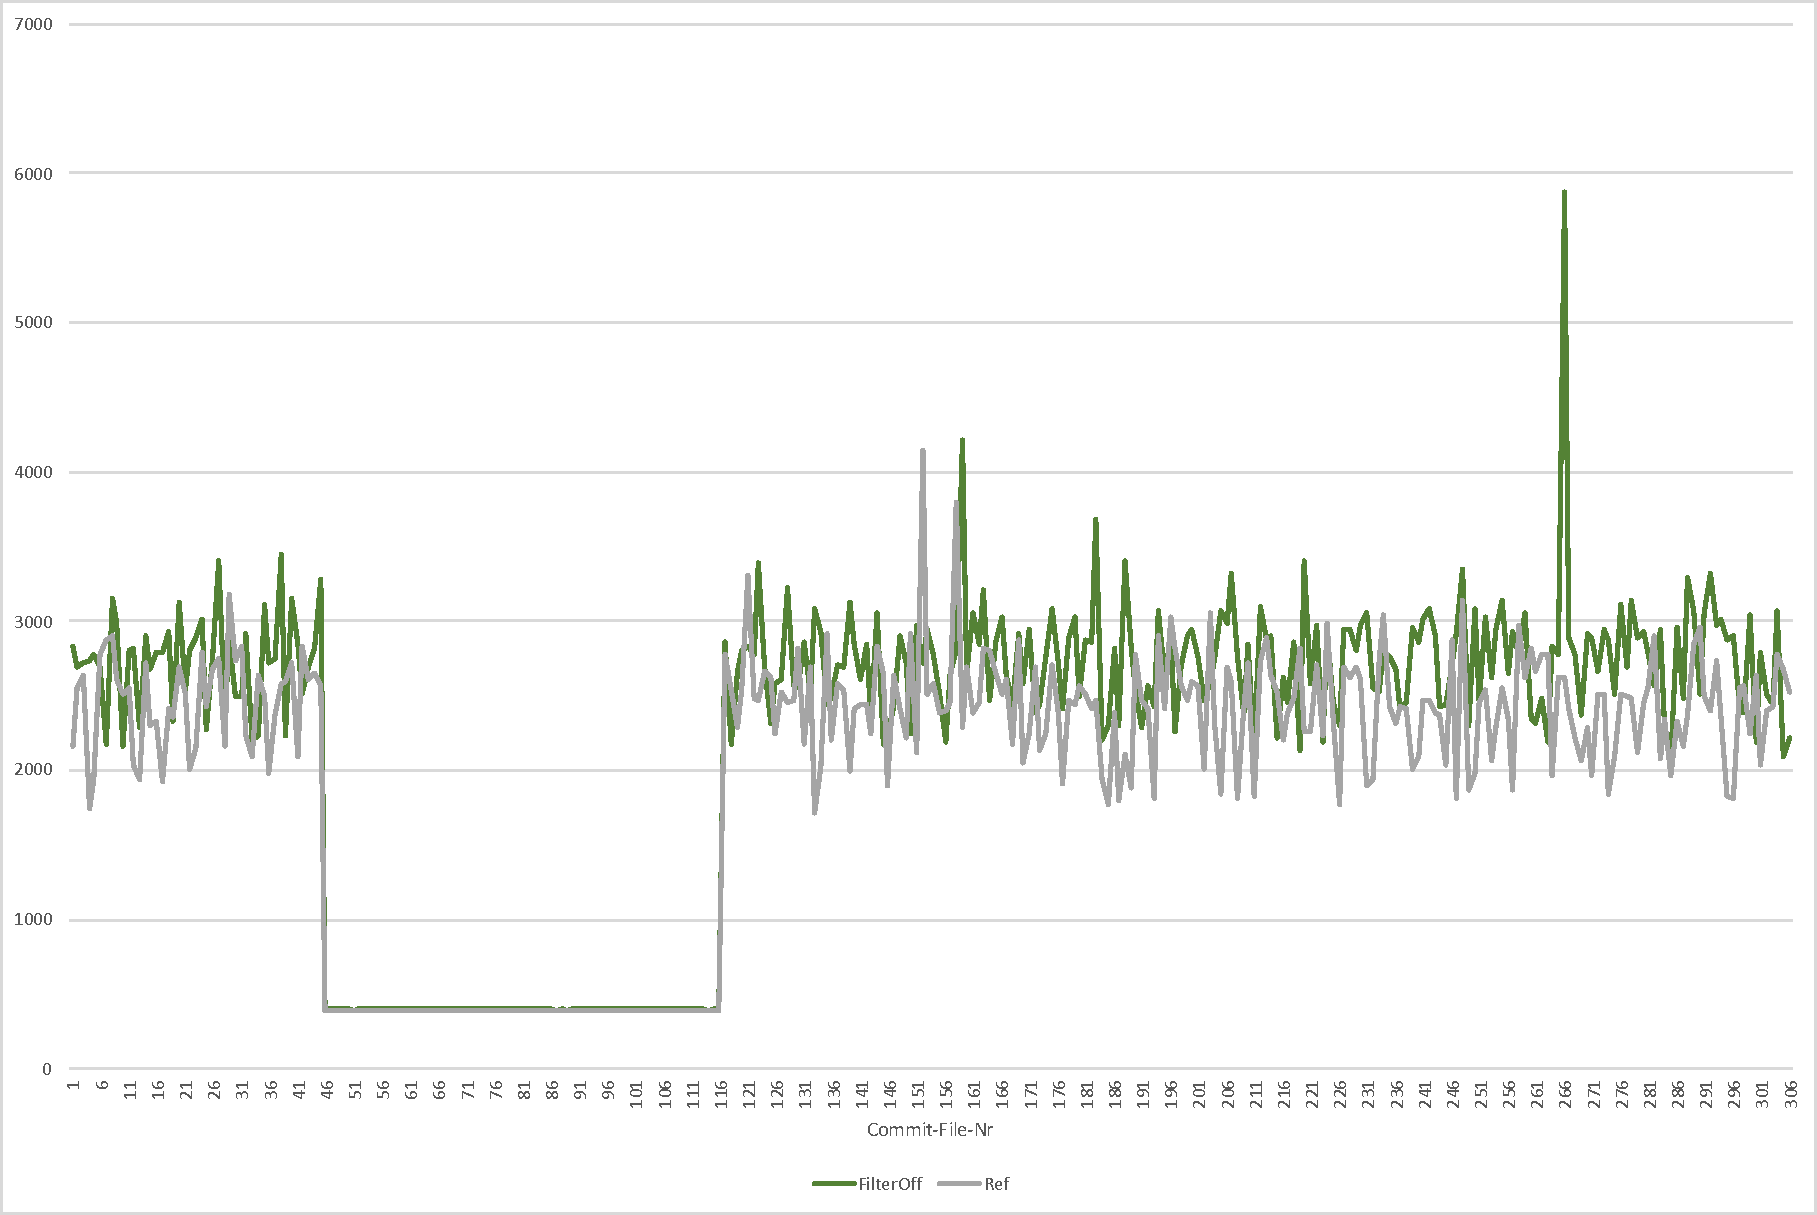
\includegraphics[height=1\textwidth, angle=90]{img/filteroff-vs-ref.pdf}
  \end{minipage}
\end{figure}


\autoref{fig:filteroff-vs-ref} shows the individual results of FilterOff and Ref in comparision. Overall, the plot does not reveal any unexpected values. Apart from one outlier that is most likely due to reasons outside of our implementation (similar to the outlier within ChangeOnly), the execution times are compareable between FilterOff and Ref executions. For the range of commits affected by the \texttt{KConfigReaderExtractor} bug, the execution times match almost exactly. As both the Preparation-Phase and Post-Extraction Phase do not introduce any noteworthy overhead, the computations for Ref and FilterOff within that range are fairly similar. The extractors are started and run until they terminate. Subsequently, the analysis notices that not all models are available and therefore terminates. As the analysis does not actually perform any computation on the models, those executions are free of randomization effects of the SAT-Solver resulting in the curve almost being linear and parallel to the y-axis.

\clearpage
\newpage

\section{Threats to Validity}\label{threats-to-validity}

During the evaluation we used configuration files for KernelHaven that were largely taken over from existing configurations for non-incremental analyses. Those configurations were known to work with KernelHaven in general. More specifically we only worked with \texttt{*.c} files for the code model as this is the default setting as implemented within KernelHaven\footnote{as defined by the default value for \texttt{code.extractor.file\_regex} in \url{https://github.com/KernelHaven/KernelHaven/blob/master/src/net/ssehub/kernel_haven/config/DefaultSettings.java}}. Eventhough the incremental infrastructure is able to handle \texttt{*.h} files just as well with the UndertakerExtractor, we have not specifically tested a configuration which includes them for extraction and analysis. To overcome this threat to \emph{internal validity}, a repeated evaluation with multiple alternative configuration files would have been desirable but was not performed due to the lack of time until the deadline of this work.

The evaluation has been performed on a subset of input files that cover about three months of the development within the Linux Kernel project. To further increase  \emph{conclusion validity} it would be desirable to repeat the evaluation with a larger set of input files. Furthermore, we already experienced one outlier within our evaluation that we investigated by repeating the execution of the analysis for a specific part of our evaluation results. This example shows that  performance results vary for individual analyses based on the same git-diff file which imposes a further threat to \emph{conclusion validity}.

We implemented the dead code analysis as one analysis within an infrastructure that can potentially be used for other analyses as well. As our evaluation only covered a very specific analysis, it remains to be seen whether implementations of other analyses within our infrastructure can produce a similar performance benefit. Because our findings are only based on one analysis and might not be transferrable to other analyses, this imposes a threat to \emph{external validity}.


\clearpage
\newpage
\section{Conclusion}\label{conclusion}

In this work, we described an approach to improve the performance of analyses of software product lines. Our approach introduces incremental analyses that work based on the newly introduced changes to a product line instead of reanalyzing the entire codebase. Our implementation of an incremental dead code analysis demonstrates siginificant improvements to performance. Overall, we were able to achieve roughly between $5\times$ to $10\times$ the performance of the reference system while still obtaining consistent results. 
In fact, most executinos of our incremental analyses only took a few seconds to finish. The largest leaps in performance were achieved by partial analyses that only processed updated parts of the code model. The results of such partial analyses reliably provided the same information about variability related dead code blocks that was gained by performing a full analysis in the reference system.

Through the reduced computational for analysis executions, our approach enables more frequent analyses on software product lines and for most executions even timely feedback for develpers within seconds. However we still do have performance spikes in instances where a more substantial part of the software product line needs to be analyzed in about 10\% to 20\% of executions. While the perfomance in such situations is still compareable with the reference system, it is significantly higher than other executions of our incremental dead code analysis. In fact those spikes made up 99\% of the duration required for all analyses on our evaluation dataset. Future research focusing on the reduction of the duration or frequency of such performance spikes would allow even better versatility for performing analyses in the context of CI or the application of software product line analyses on less powerful computer systems like developer workstations or laptops.
Additionally the implementation of incremental analyses other than the dead code analysis could be useful for investigating whether the concept of incrmenental analyses is transferrable to other analysis types.

%\Bibliography
\clearpage
\newpage

\bibliography{sources}

\clearpage
\newpage
\appendix
\section{Appendix}
\subsection{Manual for Incremental Infrastructure}

This section explains the setup and configuration of the incremental analysis for the execution of incremental analyses. Furthermore a short overview of the extension possiblities of the infrastructure  is provided for developers.

\subsubsection{Setup}

For the setup we assume that the KernelHaven infrastructure has already been set up according to its documentation\footnote{https://github.com/KernelHaven/KernelHaven/wiki/Setup-and-Execution}.
For the incremental infrastructure, you additionally need to download the current jar-files of the following projects and place them in the plugin directory:

\begin{itemize}
	\item \texttt{IncrementalAnalysesInfrastructure} 
	\item \texttt{ComAn}
\end{itemize}

If you want to use the incremental dead code analysis, you also need to add the following additional jar-files of the following projects to the plugin folder:

\begin{itemize}
	\item \texttt{IncrementalDeadCodeAnalysis}
	\item \texttt{UnDeadAnalyzer}
	\item \texttt{CnfUtils} 
\end{itemize}

Additionally, you need to prepare an empty folder that can be used for the \texttt{HybridCache}. 

\subsubsection{Configuration and Execution}

In order to use the incremental infrastructure, it is important to use an Analysis that contains the \texttt{Incremental\-Post\-Extraction} as analysis component. Furthermore \texttt{Incremental\-Preparation} must be configured as Preparation-Plugin. Code, build and variability model files can individually be filtered using the \texttt{Change\-Filter}, \texttt{Default\-Filter} or \texttt{Variability\-Change\-Filter} that were introduced in Section \ref{preparation-phase}. All three filters use a regular expression in order to determine which files represent which model. Those regular expressions can also be configured within the configuration-file. The \texttt{Variability\-Change\-Filter} requires that \texttt{Variability\-Diff\-Analyzer} is used as the diff analyzer class. The \texttt{Simple\-Diff\-Analyzer} can be used if \texttt{Variability\-Diff\-Analyzer} is not used for any of the models.

A rollback can be achieved by adding the line \texttt{incremental.rollback = true} to the configuration and then starting KernelHaven based on that configuration. KernelHaven will then perform a rollback on the HybridCache and revert the changes described by the git-diff file that is referenced from within the configuration-file.

The execution itself is started as usual for KernelHaven:

\texttt{\$ java -jar KernelHaven.jar configuration.properties}

The following configuration snippet shows all configuration options that are relevant for incremental analyses specifically. For brevety, all classes are referred to by their simple name instead of their fully qualified class name. Detailed examples of working configurations can be found in Section \ref{config-evaluation}

\begin{lstlisting}[language=java]
# Analysis class
analysis.class = IncrementalDeadCodeAnalysis
# Directory for the Hybrid Cache
incremental.hybrid_cache.dir = hybrid_cache/
# Path to git-diff file that is used as input
incremental.input.source_tree_diff = git.diff
# Set IncrementalPreparation as preparation class
preparation.class.0 = IncrementalPreparation

# InputFilter classes and DiffAnalyzer class
incremental.code.diff_analyzer_class = SimpleDiffAnalyzer
incremental.code.filter = ChangeFilter
incremental.build.filter = DefaultFilter
incremental.variability.filter = VariabiltyChangeFilter

# These regular expressions are used to assign artifacts within
# the codebase to the code, variability or build model  
code.extractor.file_regex = .*\.c
variability.extractor.file_regex = .*(?i)(^|\/|\\)(Kconfig)
build.extractor.file_regex = .*(?i)(^|\/|\\)(Makefile\.?\w*|Kbuild|Build)
\end{lstlisting}

\subsubsection{Extension of the Incremental Infrastructure}

The incremental infrastructure supports custom impelemtations of incremental analyses. An incremental analysis either works using the \texttt{Hybid\-Cache\-Adapter} as explained in Section \ref{incremental-analyses} or alternatively is implemented as an \texttt{Analysis\-Component} that can directly process an \texttt{Hybrid\-Cache}-object as input. For the latter, the analysis needs to be configured within an AnalyisisPipeline where the \texttt{Incremental\-Post\-Extraction} is the first component.

Custom filtering options can be created by creating implementations of the abstact \texttt{InputFilter} class. Finally one could also create replacements for the \texttt{SimpleDiffAnalyzer} or \texttt{VariabilityDiffAnalyzer}. However such an implementation should at least flag commit entries as \texttt{MODIFICATION}, \texttt{DELETION} or \texttt{ADDITION}.


\subsection{KernelHaven Configurations used for Evaluation} \label{config-evaluation}
This section lists the most relevant settings used for the evaluation of the incremental infrastructure and the incremental dead code analysis. For brevety only the names of the classes are used instead of the fully qualified class names required by KernelHaven. For every configuration, reading and writing to the KernelHaven cache was deactivated and all timeout options were set to 0.

\subsubsection{Ref configuration}

This is the configuration used to generate the results of a non-incremental dead code analysis as the baseline to compare against for all incremental analyses.

\begin{lstlisting}[language=java]
# General
resource_dir = res/
output_dir = output/incremental/
plugins_dir = plugins/
archive = false
archive.dir = archive/incremental
log.dir = log/incremental/
log.console = false
log.file = true
log.level = DEBUG
source_tree = source-code/linux/
arch = x86

# Analysis  
analysis.class =  ThreadedDeadCodeAnalysis
analysis.undead.threads = 20

# Extractors  
code.extractor.class = UndertakerExtractor
code.extractor.file_regex = .*\.c
code.extractor.parse_to_ast = true
code.extractor.threads = 1
code.extractor.process_ram = 10G
code.extractor.fuzzy_parsing = true
build.extractor.class = KbuildMinerExtractor
variability.extractor.class = KconfigReaderExtractor
\end{lstlisting}

\clearpage


\subsubsection{Change configuration}

This is the configuration used to evaluate the execution of the incremental dead code analysis according to the \texttt{change-only} option described in  REQ \ref{req:mandatory-filters}.

\begin{lstlisting}[language=java]
# General
resource_dir = res/
output_dir = output/incremental/
plugins_dir = plugins/
archive = false
archive.dir = archive/incremental
log.dir = log/incremental/
log.console = false
log.file = true
log.level = DEBUG
source_tree = source-code/linux/
arch = x86

# Analysis  
analysis.class = IncrementalThreadedDeadCodeAnalysis
incremental.hybrid_cache.dir = hybrid_cache/
incremental.input.source_tree_diff = xxxxx-git.diff
preparation.class.0 = IncrementalPreparation
analysis.undead.threads = 20

incremental.code.diff_analyzer_class = SimpleDiffAnalyzer
incremental.code.filter = ChangeFilter
incremental.build.filter = ChangeFilter
incremental.variability.filter = ChangeFilter

# Extractors  
code.extractor.class = UndertakerExtractor
code.extractor.file_regex = .*\.c
code.extractor.parse_to_ast = true
code.extractor.threads = 1
code.extractor.process_ram = 10G
code.extractor.fuzzy_parsing = true
build.extractor.class = KbuildMinerExtractor
variability.extractor.class = KconfigReaderExtractor
\end{lstlisting}

\clearpage

\subsubsection{VarChange configuration}

This is the configuration used to evaluate the execution of the incremental dead code analysis according to the \texttt{variability-change-only} option described in  REQ \ref{req:mandatory-filters}.

\begin{lstlisting}[language=java]
# General
resource_dir = res/
output_dir = output/incremental/
plugins_dir = plugins/
archive = false
archive.dir = archive/incremental
log.dir = log/incremental/
log.console = false
log.file = true
log.level = DEBUG
source_tree = source-code/linux/
arch = x86

# Analysis  
analysis.class = IncrementalThreadedDeadCodeAnalysis
incremental.hybrid_cache.dir = hybrid_cache/
incremental.input.source_tree_diff = xxxxx-git.diff
preparation.class.0 = IncrementalPreparation
analysis.undead.threads = 20

incremental.code.diff_analyzer_class = VariabilityDiffAnalyzer
incremental.code.filter = VariabilityChangeFilter
incremental.build.filter = VariabilityChangeFilter
incremental.variability.filter = VariabilityChangeFilter

# Extractors  
code.extractor.class = UndertakerExtractor
code.extractor.file_regex = .*\.c
code.extractor.parse_to_ast = true
code.extractor.threads = 1
code.extractor.process_ram = 10G
code.extractor.fuzzy_parsing = true
build.extractor.class = KbuildMinerExtractor
variability.extractor.class = KconfigReaderExtractor
\end{lstlisting}

\clearpage

\subsubsection{FilterOff configuration}

This is the configuration used to evaluate the execution of the incremental dead code analysis according to the \texttt{off} option described in  REQ \ref{req:mandatory-filters}.

\begin{lstlisting}[language=java]
# General
resource_dir = res/
output_dir = output/incremental/
plugins_dir = plugins/
archive = false
archive.dir = archive/incremental
log.dir = log/incremental/
log.console = false
log.file = true
log.level = DEBUG
source_tree = source-code/linux/
arch = x86

# Analysis  
analysis.class = IncrementalThreadedDeadCodeAnalysis
incremental.hybrid_cache.dir = hybrid_cache/
incremental.input.source_tree_diff = xxxxx-git.diff
preparation.class.0 = IncrementalPreparation
analysis.undead.threads = 20

incremental.code.diff_analyzer_class = SimpleDiffFilter
incremental.code.filter = DefaultFilter
incremental.build.filter = DefaultFilter
incremental.variability.filter = DefaultFilter

# Extractors  
code.extractor.class = UndertakerExtractor
code.extractor.file_regex = .*\.c
code.extractor.parse_to_ast = true
code.extractor.threads = 1
code.extractor.process_ram = 10G
code.extractor.fuzzy_parsing = true
build.extractor.class = KbuildMinerExtractor
variability.extractor.class = KconfigReaderExtractor
\end{lstlisting}

\clearpage

\subsection{Satisfied Requirements}

\begin{longtable}{ |  L{0.17\textwidth} | C{0.12\textwidth} | L{0.63\textwidth} |}
	\hline
	\textbf{Requirement} & \textbf{Satisfied} & \textbf{Comment} \\
	\hline
	REQ \ref{req:working-base} & \cmark & The incremental infrastructure processes a change in form of a git-diff file (see REQ \ref{req:git-diff}). The introduce change is used in conjunction with a folder containing the previous state of the codebase. \\ \hline
	REQ \ref{req:git-diff} & \cmark & The incremental infrastructure processes a git-diff file as input. The git-diff file must be generated using the following git diff command: \texttt{git diff --no-renames --binary commitHashA commitHashB} \\ \hline
	REQ \ref{req:analysis-types} & \cmark & The incremental infrastructure is able to handle block based analyses as demonstrated through the implementation of the dead code analysis (see REQ \ref{req:dead-code-analysis}. \\ \hline
	REQ \ref{req:early-filtering} & \cmark & Through \texttt{InputFilters} which are applied in the Preparation-Phase the incremental infrastructure supports the filtering of extractor input. \\ \hline
	REQ \ref{req:partial-models} & \cmark & \texttt{Hybrid\-Cache} provides access to the previous and current models thereby allowing analyses to selectively use parts of the models. Furthermore, \texttt{Hybrid\-Cache\-Adapter} includes options for providing a partial or complete code model. \\ \hline
	REQ \ref{req:optimization} & \cmark &  Different filtering methods can be configured within the configuration-file by defining an implementation of \texttt{InputFilter}-class as filter. \\ \hline
	REQ \ref{req:mandatory-filters} & \cmark &  The filter options \texttt{off}, \texttt{change-only} and \texttt{variability-change-only} can be achieved using the \texttt{Defaultfilter}, \texttt{ChangeFilter} and \texttt{VariabilityChangeFilter} as  \texttt{InputFilter} \\ \hline
	REQ \ref{req:effect-filters} & \xmark &  could not be implemented before deadline\\ \hline
	REQ \ref{req:rollback} & \cmark & Implemented through \texttt{Hybrid\-Cache} and the \texttt{DiffApplyUtil}-class. A rollback can be executed by adding \texttt{incremental.rollback = true} to the configuration-file of an incremental analysis and then executing KernelHaven with the configuration. \\ \hline
	REQ \ref{req:format} & \cmark & The result of the implemented incremental dead code analysis has the same file format as the non incremental dead code analysis\\ \hline
	REQ \ref{req:coverage} & \cmark & The result of the dead code analysis only contains dead code blocks that were found as a result of the current analysis execution.\\ \hline
	REQ \ref{req:target-artifacts} & \cmark & The incremental infrastructure does allow extractors to work with any type of file. The \texttt{VariabilityChangeFilter} also fulfills REQ \ref{req:target-artifacts}  but is specifically tailored towards the files within the codebase of the Linux Kernel.\\ \hline
	REQ \ref{req:existing-analyses} & \cmark & Existing \texttt{AnalysisComponents}  can be reused using the \texttt{Hybrid\-Cache\-Adapter}.\\ \hline


	
\end{longtable}



\end{document} 